\documentclass[12pt,a4paper]{report}
\usepackage[utf8]{inputenc}
\usepackage[T1]{fontenc}
\usepackage{mathpazo}
\usepackage[margin=2.5cm]{geometry}
\usepackage{graphicx}
\usepackage{booktabs}
\usepackage{amsmath,amssymb}
\usepackage{hyperref}
\usepackage{natbib}
\usepackage{caption}
\usepackage{float}
\usepackage{longtable}
\usepackage{enumitem}
\usepackage{xcolor}
\usepackage{tabularx}
\usepackage{multirow}
\usepackage{tikz}
\usetikzlibrary{positioning,arrows.meta,shapes.geometric,fit}

\bibliographystyle{plainnat}

\hypersetup{
  colorlinks=true,
  linkcolor=blue!60!black,
  citecolor=blue!60!black,
  urlcolor=blue!60!black
}

\title{\textbf{HYDRA: Explainability-Driven Intrusion Detection\\for IoT Network-Flow Data}}
\author{Varatt Saengsiripongpun\\[1em]
Bachelor of Science (Honours) in\\Computer Science and Artificial Intelligence\\[1em]
The University of Bath\\[1em]
2026}
\date{}

\begin{document}

% ============================================================
% TITLE PAGE
% ============================================================
\begin{titlepage}
\centering
\vspace*{2cm}
{\LARGE\bfseries HYDRA: Explainability-Driven Intrusion Detection\\[0.3em] for IoT Network-Flow Data\par}
\vspace{2cm}
{\Large Varatt Saengsiripongpun\par}
\vspace{1.5cm}
{\large Bachelor of Science (Honours) in\\Computer Science and Artificial Intelligence\par}
\vspace{1.5cm}
{\large The University of Bath\par}
\vspace{1cm}
{\large 2026\par}
\vfill
{\normalsize CM32017 Individual Project\par}
\end{titlepage}

% ============================================================
% COPYRIGHT
% ============================================================
\newpage
\thispagestyle{empty}
\section*{Copyright}
Attention is drawn to the fact that copyright of this dissertation rests with its author. The Intellectual Property Rights of the products produced as part of the project belong to the author unless otherwise specified below, in accordance with the University of Bath's policy on intellectual property.

This copy of the dissertation has been supplied on condition that anyone who consults it is understood to recognise that its copyright rests with its author and that no quotation from the dissertation and no information derived from it may be published without the prior written consent of the author.

\section*{Declaration}
This dissertation is submitted to the University of Bath in accordance with the requirements of the degree of Bachelor of Science in the Department of Computer Science. No portion of the work in this dissertation has been submitted in support of an application for any other degree or qualification of this or any other university or institution of learning. Except where specifically acknowledged, it is the work of the author.

% ============================================================
% ABSTRACT
% ============================================================
\newpage
\begin{abstract}
Machine-learning-based Intrusion Detection Systems (IDS) achieve high benchmark performance yet frequently operate as opaque black boxes, issuing alerts without reliable justification. This opacity creates direct operational costs: analysts must investigate alerts without trustworthy guidance, false positives generate alert fatigue, and trust in automated detection degrades even when headline accuracy is strong.

This dissertation presents HYDRA, an explainability-driven IDS framework that treats model explanations as measurable system outputs. HYDRA addresses two tasks simultaneously: binary attack detection and multi-class attack-type classification, reflecting the operational need to know both that an anomaly has occurred and which threat category it represents. The core model set comprises majority-class and threshold baselines, Logistic Regression (as a reference explainer), Random Forest, XGBoost, and LightGBM, evaluated on TON\_IoT as the primary benchmark and CIC-IoT-2023 for generalisation. A CNN-LSTM model is fully implemented as a deep learning extension; a Graph Neural Network is fully implemented with GraphSAGE and Integrated Gradients attribution.

Explanations are generated using a portfolio of post-hoc methods matched to each model family: SHAP TreeExplainer for the tree ensembles, SHAP LinearExplainer for Logistic Regression, and LIME applied model-agnostically across all models. Integrated Gradients is implemented for the CNN-LSTM and GNN extensions. Every explanation method is evaluated against five measurable criteria: faithfulness (comprehensiveness and sufficiency under top-$k$ feature ablation), stability (Spearman rank correlation under noise perturbation and across independent retraining runs), simplicity ($k_{90}$ fraction and Gini coefficient), plausibility (RMA@$k$ against expert network features), and timeliness (milliseconds per sample). Identifier-based leakage from IP addresses and port numbers is controlled through two explicit feature regimes.

The contribution is not a novel detection algorithm but a reproducible evaluation framework that operationalises explainability as a measurable system property, enabling rigorous assessment of whether high-performing IDS models can provide explanations that are faithful, stable, and useful enough to support analyst decision-making in practice.

On TON\_IoT, all four tabular models achieve PR-AUC of 1.000 and ROC-AUC of 1.000 under the behaviour-only regime, with XGBoost achieving the highest OXS explanation quality score of 0.828. Cross-dataset evaluation on CIC-IoT-2023 reveals that tree ensemble models suffer catastrophic ROC-AUC drops of up to 87\%, while Logistic Regression generalises most robustly (ROC-AUC drop of 7.3\%). The leakage interaction analysis demonstrates that including identifier features reduces explanation plausibility by 35 percentage points (Cohen's $d = -2.985$) without affecting detection performance.
\end{abstract}

% ============================================================
% ACKNOWLEDGEMENTS
% ============================================================
\newpage
\section*{Acknowledgements}
I would like to express my sincere gratitude to my supervisor, Dr Julian Padget, for his expert guidance, detailed feedback, and sustained encouragement throughout this project. His interdisciplinary perspective across artificial intelligence, formal methods, and security systems has been invaluable in shaping the scope and rigour of this work.

I am grateful to the Department of Computer Science at the University of Bath for the academic environment and computational resources that supported this research.

I also thank the research communities behind the datasets used in this project---particularly the UNSW Canberra Cyber Security Group for the TON\_IoT dataset and the Canadian Institute for Cybersecurity for CIC-IoT-2023---whose publicly available resources form the empirical foundation of this dissertation.

Finally, I acknowledge the use of generative AI tools for text editing and structural suggestions during the drafting process, in accordance with the University of Bath's Type B guidelines on AI-assisted assessment. All technical ideas, design decisions, experimental methodology, analysis, and written conclusions are the author's own work.

% ============================================================
% TABLE OF CONTENTS
% ============================================================
\tableofcontents
\listoftables
\listoffigures

% ============================================================
% CHAPTER 1: INTRODUCTION
% ============================================================
\chapter{Introduction}
\label{ch:introduction}

\section{Motivation}
\label{sec:motivation}

The cyber-defence landscape of 2025 is defined by a fundamental asymmetry: defenders must secure an ever-expanding and heterogeneous attack surface, while adversaries require only a single successful compromise. This imbalance is sharpening rapidly. Industrial-scale automated scanning and exploitation infrastructure now operates at tens of thousands of scans per second, and credential-based attacks have risen markedly in recent years \citep{fortinet2025}. Simultaneously, enterprises generate billions of log and telemetry events per day across servers, endpoints, cloud services, and IoT devices, creating a signal-to-noise problem that overwhelms both traditional rule-based monitoring and human analysts working at scale \citep{dang2023}.

Conventional security controls---signature-based Intrusion Detection Systems (IDS), rule-driven Security Information and Event Management (SIEM) platforms, and manual incident triage---were never designed for this operating environment. Signature-based systems such as Snort and Suricata offer high precision for known threats but are fundamentally reactive: they cannot detect previously unseen attacks, polymorphic malware, or adversaries who operate using legitimate credentials and living-off-the-land techniques \citep{ahmad2021}. SIEM platforms aggregate and correlate events but depend on static rule sets whose maintenance overhead grows with system complexity, and which produce high false positive rates when alert thresholds are set conservatively \citep{zhu2023}.

The emerging discipline of AIOps for cybersecurity seeks to address these limitations by embedding machine learning, automation, and streaming analytics into the Security Operations Centre (SOC). Industry analyses suggest that mature AIOps platforms can reduce alert noise by 70--90\% through automated correlation and deduplication, and can significantly improve mean time to detect (MTTD) and mean time to respond (MTTR) to incidents \citep{dang2023,nguyen2024}. However, the adoption of learned models introduces new operational challenges: deep learning systems frequently behave as opaque black boxes; real-time inference at SOC scale imposes strict latency constraints; and models are vulnerable to concept drift and adversarial manipulation in hostile environments \citep{schwarzschild2021,goldblum2023}.

\section{Problem Statement}
\label{sec:problem}

A central failing of current IDS research is the gap between detection performance and operational usefulness. High benchmark accuracy on public datasets does not translate directly into deployable, trustworthy systems for three interconnected reasons.

First, many published results are inflated by evaluation leakage. When network-flow records are split randomly by row, highly similar traffic from the same hosts, sessions, or adjacent time windows appears in both training and test sets, allowing models to achieve near-perfect scores by recognising identity patterns---specific IP addresses, port combinations, or session fingerprints---rather than learning attack behaviour \citep{turcotte2017}. This type of leakage is invisible under standard evaluation but would cause catastrophic performance degradation in deployment against unseen infrastructure.

Second, most IDS models provide binary outputs---attack or normal---without indicating which category of threat has been detected. In practice, different attack types such as denial-of-service, ransomware, data exfiltration, and scanning require different analyst responses and escalation paths. A system capable of both binary detection and multi-class attack-type classification is therefore substantially more operationally useful.

Third, even accurate models are frequently dismissed or underutilised because their alerts lack justification. When a model flags a flow as malicious without explaining which behavioural features triggered the decision, analysts must investigate blindly. This increases mean time to triage, compounds alert fatigue, and erodes the trust required for automation to be accepted in high-stakes SOC environments.

\section{Aim and Objectives}
\label{sec:aim}

The aim of this project is to design, implement, and evaluate HYDRA: an intrusion detection framework that addresses both binary attack detection and multi-class attack-type classification, while generating per-alert explanations that are systematically validated for reliability, consistency, and operational usefulness on IoT network-flow data.

The specific objectives are:
\begin{enumerate}
  \item To implement and evaluate a structured model progression---from baselines through tabular ensemble models---for both binary and multi-class intrusion detection on TON\_IoT, with CIC-IoT-2023 as a secondary generalisation benchmark. A CNN-LSTM model is additionally fully implemented as a deep learning extension; a Graph Neural Network is fully implemented with GraphSAGE and Integrated Gradients attribution.
  \item To define and apply two feature regimes that explicitly isolate and quantify the contribution of identifier leakage to detection performance and explanation quality.
  \item To generate standardised per-alert explanation records for tabular models using SHAP TreeExplainer, for the Logistic Regression reference model using SHAP LinearExplainer, and for all models using LIME as a model-agnostic cross-reference. Integrated Gradients is implemented for the CNN-LSTM and GNN extensions.
  \item To evaluate explanations systematically using five measurable criteria: faithfulness (comprehensiveness and sufficiency), stability (under noise perturbation and across independent retraining seeds), simplicity ($k_{90}$ and Gini), plausibility (RMA@$k$), and timeliness (ms per sample).
  \item To position HYDRA explicitly against concurrent XAI-IDS work and compare the performance--explainability trade-off across model types, with generalisation evaluation on CIC-IoT-2023 where feasible.
\end{enumerate}

\section{Research Questions}
\label{sec:rqs}

This project is structured around four research questions:

\noindent\textbf{RQ1 (Detection):} Which modelling approach provides the strongest performance for both binary attack detection and multi-class attack-type classification on tabular network-flow features, when evaluated using operationally relevant metrics such as PR-AUC and false positive rate at a fixed recall target?

\noindent\textbf{RQ2 (Explainability):} To what extent can the best-performing detector provide per-alert, feature-level explanations with high and consistent coverage across both detection tasks?

\noindent\textbf{RQ3 (Reliability):} How stable are explanation outputs across repeated training runs and different data conditions, and does stability differ between the binary and multi-class tasks?

\noindent\textbf{RQ4 (Faithfulness):} Do model-generated explanations exhibit fidelity---that is, does removing the highlighted features significantly change model confidence---and do explanation patterns align with known network intrusion behaviours for each attack type?

\section{Contributions}
\label{sec:contributions}

This project does not propose a novel detection algorithm. Its contributions are:
\begin{itemize}
  \item A reproducible IDS pipeline that supports both binary and multi-class intrusion detection with standardised per-alert explanation records for tabular ensembles, with a CNN-LSTM extension fully implemented for deep learning evaluation.
  \item A unified, implementation-ready explainability evaluation protocol covering five measurable criteria (faithfulness, stability, simplicity, plausibility, timeliness), applied consistently across all evaluated model families and both detection tasks. Importantly, the stability criterion is operationalised as two separate experiments: seed-retraining stability (training $S = 5$ models with different random seeds) and noise-perturbation robustness (perturbing fixed model inputs), which address distinct aspects of explanation reliability.
  \item Empirical analysis of the impact of identifier-based feature leakage on detection performance and explanation quality in IoT network-flow datasets, and explicit positioning of HYDRA against concurrent XAI-IDS systems through a gap analysis table.
\end{itemize}

\section{Dissertation Structure}
\label{sec:structure}

Chapter~\ref{ch:literature} presents the literature, technology, and data survey, covering the evolution of intrusion detection and AIOps, supervised and unsupervised learning for cyber defence, deep learning approaches to log and flow analysis, predictive analytics, explainability methods, and a critical survey of the datasets used. Chapter~\ref{ch:methodology} describes the HYDRA methodology. Chapter~\ref{ch:results} presents experimental results. Chapter~\ref{ch:discussion} discusses findings, trade-offs, and limitations. Chapter~\ref{ch:conclusions} concludes and identifies future work. A full bibliography and appendices follow.

% ============================================================
% CHAPTER 2: LITERATURE REVIEW
% ============================================================
\chapter{Literature, Technology and Data Survey}
\label{ch:literature}

\section{Introduction}
\label{sec:lit-intro}

This chapter reviews the literature, technology landscape, and available datasets relevant to HYDRA. Section~\ref{sec:evolution} traces the evolution of intrusion detection from signature-based systems through machine-learning anomaly detection to AIOps. Section~\ref{sec:supervised} examines supervised and unsupervised learning algorithms used in cyber defence. Section~\ref{sec:deeplearning} covers deep learning approaches to log and network-flow analysis. Section~\ref{sec:graphbased} reviews predictive analytics for cyber threats. Section~\ref{sec:xai} surveys explainability methods, with particular focus on post-hoc feature attribution and graph-based explanation. Section~\ref{sec:gaps} identifies critical gaps in existing technology that motivate HYDRA's design. Section~\ref{sec:techsurvey} surveys key technologies used in the implementation. Section~\ref{sec:datasurvey} surveys the datasets used in evaluation.

\section{Evolution of Intrusion Detection: From Signatures to AIOps}
\label{sec:evolution}

\subsection{Signature-Based and Rule-Based Systems}
\label{sec:signature}

Early intrusion detection technology was dominated by signature-based systems such as Snort and Suricata, which compare packet headers and payloads against libraries of known Indicators of Compromise (IoCs). These systems offer high precision for threats whose signatures are already catalogued and low computational overhead. However, their fundamental limitation is their inability to detect previously unseen attacks. Signature databases must be manually maintained, and any attack variant that differs from the known pattern---through obfuscation, encryption, or minor modification---will evade detection entirely. As adversaries increasingly rely on encrypted channels, legitimate system tools, and credential theft rather than novel exploits, the coverage of static signatures continues to erode \citep{ahmad2021}.

Rule-based SIEM platforms extend signature detection by correlating events across sources and applying logic rules to identify multi-step attack sequences. However, \citet{zhu2023} highlight that as software complexity increases, static parsing rules become brittle: they require continuous manual update, generate high false positive rates when applied to heterogeneous modern telemetry, and miss anomalies that do not match any predefined pattern. The maintenance burden of rule sets scales poorly with the diversity and volume of data produced by modern enterprise and IoT environments.

\subsection{Anomaly-Based Detection and Machine Learning}
\label{sec:anomaly}

To address the zero-day detection gap, research shifted towards anomaly-based IDS, where models learn a statistical baseline of normal behaviour and flag deviations. Early statistical methods such as threshold-based detection and principal component analysis provided a foundation, but their performance was limited on high-dimensional, non-linear network traffic data.

The application of machine learning to IDS marked a significant advance. Supervised approaches such as Random Forest, Support Vector Machines, $k$-Nearest Neighbours, and gradient boosting methods demonstrated high accuracy on benchmark datasets such as KDD Cup 99, NSL-KDD, and CICIDS2017 when applied to engineered flow features \citep{aldweesh2020}. These models benefit from interpretable feature importance scores and mature implementations, making them competitive baselines that remain difficult to surpass in tabular settings even with more complex architectures. However, supervised models generalise poorly to attack types not represented in training data and suffer performance degradation under concept drift as network behaviour evolves.

Hybrid IDS architectures that combine supervised classification with unsupervised anomaly detection have emerged as a research direction with particular promise. \citet{alsaedi2020} show that combining tree-based supervised models with autoencoder-based unsupervised detection on the TON\_IoT dataset yields substantially better recall on zero-day scenarios than either approach alone, while also reporting improvements in both precision and detection coverage. The hybrid modelling principle underpins HYDRA's experimental design.

\subsection{AIOps for Cybersecurity}
\label{sec:aiops}

AIOps (Artificial Intelligence for IT Operations) emerged as a broader discipline for automating IT operations through machine learning, focusing on noise reduction, automated correlation, and root-cause analysis across heterogeneous telemetry \citep{dang2023}. For cybersecurity, AIOps platforms ingest security signals from SIEMs, IDS, endpoint detection and response (EDR) systems, and cloud logging pipelines into unified analytical frameworks that operate continuously on streaming data \citep{dang2023}. Industry reports suggest that mature AIOps deployments can reduce alert noise by 70--90\% through automated deduplication and correlation, and can improve mean time to detect and mean time to respond to incidents significantly \citep{dang2023,fortinet2025}; while such figures originate from vendor analyses rather than peer-reviewed studies, the directional benefit of automated correlation is broadly supported in the research literature \citep{dang2023,zhu2023}.

Commercial AIOps and SIEM platforms from vendors including Datadog, Splunk, IBM QRadar, and CrowdStrike incorporate ML-based anomaly detection, user and entity behaviour analytics (UEBA), and increasingly, graph-based attack-path visualisation. However, these products are closed, vendor-specific, and optimised for enterprise operational metrics rather than research-grade reproducibility or publication of detailed detection and prediction benchmarks on standardised open datasets. HYDRA's contribution is a transparent, research-reproducible prototype that addresses the same operational goals while enabling rigorous empirical evaluation.

\section{Supervised and Unsupervised Learning for Cyber Defence}
\label{sec:supervised}

\subsection{Supervised Ensemble Methods}
\label{sec:ensemble}

Ensemble tree methods form the core of HYDRA's tabular detection pipeline. Random Forest \citep{breiman2001} constructs an ensemble of independently trained decision trees by combining bootstrap sampling with random feature subsets at each split, producing stable feature importance estimates well-suited to high-dimensional flow data. XGBoost \citep{chen2016} implements gradient boosted trees through second-order gradient approximation and regularisation, offering strong generalisation and efficient computation. LightGBM \citep{ke2017} extends this through histogram-based splitting for memory efficiency. Logistic Regression is also included in HYDRA's model set as a reference explainer: its linear decision boundary makes it deterministic and auditable by construction, providing a stability anchor against which the explanation reliability of the more complex ensemble models can be measured.

In the IDS literature, ensemble models consistently achieve state-of-the-art results on public benchmarks. \citet{pansare2024} integrate Restricted Boltzmann Machines, Deep Feedforward Neural Networks, LSTMs, and GRUs alongside Random Forest and XGBoost, reporting 99.9\% accuracy on CICDDoS2019 and HIKARI2021. \citet{rani2024} demonstrate that integrating Random Forest with deep artificial neural network components yields strong intrusion detection performance across multiple attack categories, outperforming standalone tree or neural network baselines. While these results appear impressive, both use datasets without explicit temporal splits, raising concerns about evaluation leakage that limit the generalisability of reported metrics.

A key challenge for supervised IDS is class imbalance. In realistic deployments, attack events represent a small fraction of total traffic. Standard accuracy metrics are therefore misleading: a classifier that always predicts normal achieves very high accuracy while detecting nothing. Operational evaluation must rely on precision-recall metrics, PR-AUC, and false positive rate at a fixed recall target, which directly reflect the burden on analysts who must investigate every raised alert.

\subsection{Isolation Forest}
\label{sec:iforest}

Isolation Forest \citep{liu2008} is a widely-used unsupervised anomaly detection algorithm well-suited to high-dimensional tabular data. Rather than profiling normal instances, it isolates anomalies directly by recursively partitioning the feature space with random cuts: anomalous points, which occupy sparse or extreme regions, require fewer partitions to isolate and receive shorter average path lengths across an ensemble of random trees. The algorithm operates in approximately linear time and memory, making it practical as a fast first-stage filter in a hybrid pipeline.

\citet{alsaedi2020} demonstrate Isolation Forest's utility as a pre-filter on the TON\_IoT dataset, showing that combining it with downstream supervised classification reduces false positives while maintaining recall comparable to supervised-only approaches. A comparative study \citep{nassif2021} confirms that Isolation Forest outperforms autoencoders for detecting point anomalies in tabular data, while autoencoders are more effective for contextual anomalies in sequential or high-dimensional embedding spaces.

\subsection{Autoencoders and LSTM-Autoencoders}
\label{sec:autoencoders}

Autoencoders are neural networks trained to compress input data into a low-dimensional latent representation and reconstruct it. When trained exclusively on normal traffic, an autoencoder learns to reconstruct normal patterns efficiently; anomalous inputs produce high reconstruction error, which serves as the anomaly score. Deep autoencoders are particularly effective for detecting subtle deviations in high-dimensional IoT telemetry data where simple threshold-based methods fail \citep{moustafa2021}.

LSTM-autoencoders extend this approach to sequential data by using Long Short-Term Memory networks as both encoder and decoder, allowing the model to capture temporal dependencies in log sequences or time-windowed traffic metrics. Studies on time-series anomaly detection demonstrate that LSTM-autoencoders can detect subtle temporal anomalies that evade point-level detection \citep{malhotra2016}. \citet{park2023} demonstrate that LSTM-autoencoders outperform classic anomaly detection baselines such as Local Outlier Factor on time-series network flow data, at the cost of higher training complexity and sensitivity to hyperparameter choices.

\section{Deep Learning for Log and Network-Flow Analysis}
\label{sec:deeplearning}

\subsection{LSTM-Based Log Analysis: DeepLog}
\label{sec:deeplog}

System logs represent structured or semi-structured text describing system state and events. The application of Natural Language Processing (NLP) techniques to log analysis has produced a series of increasingly capable models. DeepLog \citep{du2017} treats log entries as sequences of discrete log keys---templates derived by parsing variable-length log messages into fixed event identifiers---and trains an LSTM to predict the next expected key in a sequence. Deviations from the predicted key, or sequences with low predicted probability, are flagged as anomalies.

DeepLog demonstrated strong performance on the HDFS and BGL datasets from the LogHub collection \citep{zhu2023}, establishing LSTMs as a viable architecture for log-based anomaly detection. However, LSTMs are susceptible to two structural limitations: they struggle to model very long-range dependencies without careful regularisation, and they are trained unidirectionally, meaning they can only condition predictions on the left context of a sequence. As a result, DeepLog may miss anomalies that are only detectable from subsequent context.

\subsection{Transformer-Based Log Analysis: LogBERT and Variants}
\label{sec:logbert}

More recent work applies Transformer architectures to log anomaly detection. LogBERT \citep{guo2021} adapts BERT to the log domain by treating log key sequences as sentences and applying masked log key prediction as a self-supervised pre-training objective. Unlike DeepLog, LogBERT conditions each prediction on both left and right context, enabling it to detect anomalies that depend on future events. \citet{guo2021} report superior F1-scores on HDFS and BGL compared to LSTM baselines, with particular improvements in detecting anomalies involving unusual key co-occurrences.

Comparative systematic evaluations confirm that Transformer-based models achieve higher accuracy than LSTM-based approaches on LogHub benchmarks, but at substantially higher computational cost for both training and inference \citep{guo2021,le2023}. This latency--accuracy trade-off is directly relevant to real-time IDS deployment: in scenarios requiring very low detection latency, LSTM-based models or lightweight alternatives such as LogFiT \citep{qi2023} and ALogSCAN \citep{raeiszadeh2025} may be preferable.

\subsection{CNN-LSTM Ensembles for Network Flow Analysis}
\label{sec:cnnlstm-lit}

For network flow data, which has both spatial (feature interaction) and temporal (sequence) structure, hybrid CNN-LSTM architectures have been proposed to capture both dimensions simultaneously. Convolutional layers extract local feature patterns from flow-level attributes, while LSTM layers model temporal dependencies across successive time windows or flow sequences. Studies using the TON\_IoT dataset demonstrate that LSTM-based approaches---including CNN-LSTM ensembles and bidirectional LSTM variants---achieve detection accuracy above 99\% on binary classification, with strong performance maintained across multiple IoT attack types including DoS, DDoS, ransomware, and data exfiltration \citep{ferrag2022,imrana2021}.

A more recent architecture \citep{popoola2021} combines three parallel branches---CNN for spatial patterns, BiLSTM for temporal dependencies, and an autoencoder for reconstruction-error anomaly scoring---fused into a single detection model trained using federated learning. The federated approach keeps raw IoT traffic data local to each device, sharing only model updates, which addresses privacy constraints in distributed IoT environments.

\section{Graph-Based Detection and Predictive Analytics}
\label{sec:graphbased}

\subsection{Graph Neural Networks for Intrusion Detection}
\label{sec:gnn-lit}

Network communications have natural graph structure: hosts and devices are nodes, and communications between them are edges. Graph Neural Networks (GNNs) can exploit this relational structure by aggregating information from neighbouring nodes through successive message-passing operations, learning representations that capture not just individual flow features but the topology of communication patterns. This is particularly relevant for detecting attack behaviours that manifest at the graph level, such as scanning (a single source node connecting to many previously unseen destinations), lateral movement (a host establishing unusual connections to internal targets), and botnet coordination (many nodes exhibiting correlated behavioural patterns).

On the LANL dataset, temporal GNN models such as Euler \citep{king2023} and Hermes \citep{lo2023} have been applied to user authentication graphs, where nodes represent users and machines and edges represent authentication events over time. These models predict the probability of each user-machine authentication being anomalous given the historical communication topology, achieving strong performance on insider threat and lateral movement detection scenarios.

\subsection{Predictive Analytics: Forecasting Cyber Threats}
\label{sec:predictive}

Beyond detection of ongoing attacks, there is substantial interest in predicting imminent threats before they fully materialise. \citet{munkhdorj2017} propose using social data and vulnerability intelligence to estimate the probability of an impending cyber attack. Recurrent sequence models have also been applied to volumetric threat forecasting: LSTM-based approaches have been shown to forecast DDoS attack intensity up to several minutes in advance using historical traffic time series \citep{kong2025}.

Lateral movement prediction is a closely related problem with particular relevance to enterprise intrusion scenarios. Using the LANL dataset, \citet{turcotte2017} train sequence models on historical user authentication patterns to predict the next machine a user is likely to authenticate to. When a user authenticates to a machine with low predicted probability, this signals potential credential theft or lateral movement by an attacker using stolen credentials. This technique is notable because it can detect attacks that produce no direct signature---the attacker uses valid credentials and legitimate system tools---and is thus invisible to signature-based and many statistical anomaly detection approaches.

A survey of event prediction methods for cybersecurity \citep{sonmez2023} identifies three primary metrics for evaluating predictive IDS: lead time (the interval between prediction and incident), time-to-compromise estimation, and prediction reliability under class imbalance and concept drift.

\section{Explainability in Intrusion Detection}
\label{sec:xai}

\subsection{The Explainability Problem in IDS}
\label{sec:xai-problem}

High-performing ML models used for intrusion detection---particularly gradient boosted trees and deep learning architectures---frequently operate as black boxes, producing alert decisions without exposing the features or reasoning that drove them. This is problematic for several operational reasons. Analysts must investigate each alert without guidance, increasing triage time. False positives---which remain a persistent challenge even for well-performing models---are harder to identify and dismiss without understanding why the model flagged a given flow. When models are retrained or updated, analysts have no basis for assessing whether the new model has learned different or better decision rules. And in regulated sectors, security decisions may require audit trails that document the reasoning behind automated actions.

The field of Explainable AI (XAI) has developed two broad paradigms for addressing this problem. Post-hoc methods explain an already-trained model by approximating its behaviour locally or globally, without modifying the model itself. Intrinsically interpretable models are designed to be transparent by construction, at the potential cost of detection performance. For IDS, post-hoc methods are more widely used because they can be applied to high-performing ensemble and deep learning models, whereas intrinsically interpretable models such as logistic regression may not capture the non-linear patterns needed for strong detection \citep{adadi2018}.

HYDRA implements a portfolio of four complementary post-hoc explanation methods across its model set: SHAP TreeExplainer for tree-based ensemble models (Random Forest, XGBoost, LightGBM), SHAP LinearExplainer for the Logistic Regression reference model, LIME applied across all models as a model-agnostic cross-reference, and Integrated Gradients for the CNN-LSTM and GNNExplainer for the Graph Neural Network. This design allows direct comparison of explanation quality across model families and across methods applied to the same model.

\subsection{SHAP TreeExplainer: Tree Ensemble Attribution}
\label{sec:shap-tree}

SHAP (SHapley Additive exPlanations), introduced by \citet{lundberg2017}, grounds feature attribution in cooperative game theory: each feature is treated as a player in a coalition game, and its contribution to the prediction is its Shapley value---the average marginal contribution it makes across all possible orderings of features. This provides theoretically grounded attribution that satisfies efficiency, symmetry, and dummy axioms, making it the most principled and widely adopted explanation method in the IDS literature \citep{lundberg2022}.

SHAP TreeExplainer provides an exact, polynomial-time implementation specifically for tree-based models including Random Forest, XGBoost, and gradient boosted trees \citep{lundberg2020}. By exploiting the tree structure directly, TreeExplainer avoids the sampling approximation required by model-agnostic SHAP variants, making it both faster and more accurate. In HYDRA, TreeExplainer is applied to all three ensemble models and produces two types of output: local explanations that give per-alert feature contributions, and global explanations that aggregate Shapley values across the test set to produce feature importance rankings and per-attack-type heatmaps showing which features are most characteristic of each threat category.

Despite its strengths, SHAP has known limitations. Shapley values can be unstable under correlated features: when two features carry redundant information, their individual values may vary substantially across retraining even if the model's decision boundary is stable. This is addressed in HYDRA's evaluation through explicit stability measurement using Spearman rank correlation of feature importance orderings under noise perturbation.

\subsection{SHAP LinearExplainer: Logistic Regression Attribution}
\label{sec:shap-linear}

For the Logistic Regression model, SHAP LinearExplainer computes Shapley values analytically for linear models by exploiting the additive structure of linear prediction: the attribution of each feature is its coefficient multiplied by the deviation of its value from the expected value. Because Logistic Regression is a linear model, its explanations are deterministic across training runs given the same data and solver settings, making it an ideal stability anchor for comparing against the more complex tree ensemble models. The primary purpose of Logistic Regression in HYDRA is therefore as a reference explainer rather than as a competitive detector. The deviation of RF, XGBoost, and LightGBM explanations from this anchor quantifies the explainability cost of moving to more expressive models, consistent with the performance--explainability trade-off analysis of \citet{bhatt2020} and the XAI survey of \citet{adadi2018}.

\subsection{LIME: Model-Agnostic Cross-Reference}
\label{sec:lime}

LIME (Local Interpretable Model-agnostic Explanations), introduced by \citet{ribeiro2016}, explains individual predictions by sampling perturbed versions of the input, querying the model on each perturbation, and fitting a locally linear surrogate model to the resulting input-output pairs. LIME is model-agnostic and can therefore be applied identically across all of HYDRA's models, enabling direct comparison of local explanations across model families on the same alert.

HYDRA applies LIME across all models for two reasons. First, it provides a model-agnostic cross-reference against TreeSHAP and LinearSHAP attributions: significant disagreements between LIME and SHAP for the same alert indicate explanation instability that may reflect either method's limitations rather than genuine model reasoning. Second, LIME's application to the CNN-LSTM provides tabular-level local explanations that complement the gradient-based Integrated Gradients attributions applied to the same model.

LIME's primary limitation is sampling variance: the locally linear surrogate is fitted to a finite random sample of perturbations, and different samples may yield qualitatively different explanations for the same instance. Comparative studies in IDS contexts generally find SHAP to provide more stable attributions for tabular data \citep{viirlaid2025}. HYDRA therefore treats LIME as a secondary cross-reference method rather than a primary attribution source.

\subsection{Integrated Gradients: CNN-LSTM Attribution}
\label{sec:ig}

Integrated Gradients \citep{sundararajan2017} is a gradient-based attribution method for differentiable models. It computes the attribution of each input feature by integrating the model's gradients with respect to that feature along a straight-line path from a baseline input (typically a zero vector or mean-value reference) to the actual input. This integration ensures that the method satisfies sensitivity (a feature that changes the output must receive non-zero attribution) and implementation invariance (functionally equivalent models receive the same attributions regardless of implementation).

In HYDRA, Integrated Gradients is applied to the CNN-LSTM model, which combines convolutional layers for local feature pattern extraction with LSTM layers for temporal dependency modelling across time-windowed flow sequences. The CNN-LSTM and its associated explanation methods are fully implemented within HYDRA.

\subsection{GNNExplainer: Graph Neural Network Attribution}
\label{sec:gnnexplainer}

Explaining GNN predictions requires methods that account for both graph topology (which nodes and edges drove the prediction) and feature content (which attributes of those nodes and edges were decisive). GNNExplainer \citep{ying2019} addresses the topology problem by learning a soft mask over the edges of a node's computational subgraph that maximises the mutual information between the masked subgraph's prediction and the full-graph prediction, subject to a sparsity constraint. The result is a compact explanation subgraph that approximately preserves the model's prediction for the instance being explained.

GNN explanations face unique challenges not present in tabular settings. Subgraph explanations can be non-unique: multiple subgraphs may achieve equivalent mutual information with the prediction. Explanations may be dominated by graph topology rather than edge-feature content, making them uninformative about which behavioural attributes drove the detection. And unlike TreeSHAP, GNNExplainer is an optimisation-based method that introduces additional stochasticity, potentially producing different explanations across runs even for the same model and input.

HYDRA addresses this by explicitly measuring subgraph explanation stability using the same Spearman rank correlation protocol applied to other models.

\subsection{Policy Graphs and Causal Graph Explainability}
\label{sec:policy-graphs}

Beyond feature attribution, a more structured approach to IDS explainability uses graph representations of security policies and causal event chains. Policy graphs \citep{alves2017} represent access control states as directed graphs of entities and relationships, explaining alerts by identifying which entity-relationship pattern triggered a policy violation. Causal or provenance graphs represent the history of system events as dependency graphs. DepImpact \citep{fang2022} proposes backward-propagation over system dependency graphs to isolate the minimal subgraph most relevant to an observed attack. UTLParser \citep{tan2024} combines log parsing with causal graph construction for attack attribution.

HYDRA's primary explainability layer uses the post-hoc statistical methods described above, but the policy and provenance graph paradigm directly informs the plausibility evaluation criterion: explanation features that align with known policy violations or causal attack chains are considered operationally plausible, providing a domain-knowledge reference for the RMA@$k$ metric.

\subsection{XAI Evaluation: Five Criteria}
\label{sec:xai-eval}

A recurring weakness in XAI research applied to IDS is the absence of systematic evaluation of explanations. Most studies present SHAP plots or attention maps as qualitative demonstrations, without measuring whether explanations are reliable, faithful, or operationally useful. HYDRA addresses this gap by evaluating every explanation method applied to every model against five criteria, each with a specific metric, as summarised in Table~\ref{tab:five-criteria}.

\begin{table}[H]
\centering
\caption{HYDRA's five-criterion XAI evaluation framework, applied to each explanation method across each model.}
\label{tab:five-criteria}
\small
\begin{tabularx}{\textwidth}{lp{3.5cm}X}
\toprule
\textbf{Criterion} & \textbf{Metric} & \textbf{Description} \\
\midrule
Faithfulness & Comprehensiveness + Sufficiency (top-$k$ feature ablation) & Remove top-$k$ features (comprehensiveness) or keep only top-$k$ (sufficiency) and measure confidence change. High-quality explanations cause large drops when top-$k$ features are removed and small drops when only they are retained. \\
\addlinespace
Stability & S1: Spearman rank correlation across $S = 5$ independent retraining runs; S2: Spearman correlation under Gaussian input noise & Two distinct experiments. S1 measures robustness to training stochasticity (addresses RQ3). S2 measures robustness to input perturbation (addresses RQ4 robustness). Both are reported separately. \\
\addlinespace
Simplicity & $k_{90}$ fraction + Gini coefficient & $k_{90}$ is the minimum number of features needed to account for 90\% of total attribution mass, normalised by feature count. Gini coefficient measures concentration of attribution. Lower $k_{90}$ and higher Gini indicate more concise, analyst-friendly explanations. \\
\addlinespace
Plausibility & RMA@$k$ vs expert network features & Relevant-feature Match Accuracy at $k$: the proportion of top-$k$ attributed features that appear in an expert-defined reference set known to be characteristic of each attack type. \\
\addlinespace
Timeliness & Milliseconds per sample & Wall-clock time to generate a complete explanation record for a single alert. Constrains which methods are viable for real-time or near-real-time SOC deployment. \\
\bottomrule
\end{tabularx}
\end{table}

Faithfulness is measured through top-$k$ feature ablation using two complementary tests. Comprehensiveness removes the top-$k$ attributed features from the input and measures the resulting drop in model confidence. Sufficiency retains only the top-$k$ features and replaces all others with baseline values, measuring whether the retained features alone are sufficient to approximately reproduce the original confidence. Together, these provide a stronger faithfulness test than either alone \citep{bhatt2020,deyoung2020}.

Stability uses Spearman rank correlation rather than Jaccard set overlap because it captures the full ordering of feature importance---a more sensitive measure of explanation consistency---and is robust to ties. Perturbations are applied as small Gaussian noise added to continuous features, simulating the measurement noise present in real network flow monitoring. \citet{alvarez2018} demonstrate that many local explanation methods are sensitive to small changes in model parameters, producing qualitatively different explanations even when the decision boundary is largely unchanged. \citet{viirlaid2025} confirm this instability empirically in an NIDS context, finding that SHAP and LIME attributions vary meaningfully across retraining runs, reinforcing the need for HYDRA's explicit seed-retraining stability protocol.

Simplicity is quantified using two complementary measures. The $k_{90}$ fraction is the minimum number of top-attributed features needed to account for 90\% of the total attribution mass, normalised by the total feature count. The Gini coefficient of the attribution distribution measures concentration: a high Gini value indicates that attribution mass is concentrated on a small number of features, while a low value indicates diffuse attribution that is harder to interpret.

Plausibility is evaluated using Relevant-feature Match Accuracy at $k$ (RMA@$k$), computed by comparing the top-$k$ attributed features for each alert against a reference set of features that network security domain knowledge identifies as characteristic of the detected attack type. The reference sets are defined in advance from the IDS literature and used as a fixed evaluation benchmark, not tuned against model outputs.

Timeliness measures the wall-clock time required to generate a complete explanation record for a single alert at inference time, reported in milliseconds per sample. TreeSHAP is generally very fast for tree models; LIME, which requires repeated model queries for each explained sample, is substantially slower; and GNNExplainer, which solves an optimisation problem per explanation, may be the slowest. Timeliness measurement allows HYDRA to characterise these trade-offs empirically.

This five-criterion framework is applied consistently across all explanation method--model pairs in HYDRA, enabling structured comparison of explanation quality between tabular and graph models, between primary and cross-reference methods, and between the binary and multi-class detection tasks.

\section{Positioning HYDRA Against Concurrent Work}
\label{sec:positioning}

Four recent papers address XAI-IDS in settings sufficiently similar to HYDRA that explicit positioning is necessary. Table~\ref{tab:positioning} maps each paper against HYDRA's principal design choices across ten dimensions. The table makes clear that while individual components of HYDRA's approach appear in the literature, no prior work combines all of them simultaneously: dual-task detection (binary and multi-class), leakage-controlled evaluation, a five-criterion measurable XAI framework, a multi-method explanation portfolio, and cross-dataset generalisation.

\begin{table}[H]
\centering
\caption{Positioning HYDRA against concurrent XAI-IDS work. \checkmark = present, $\circ$ = partial, $\times$ = absent.}
\label{tab:positioning}
\small
\begin{tabular}{lccccc}
\toprule
\textbf{Dimension} & \textbf{HYDRA} & \textbf{E-XAI} & \textbf{XAI-IDS} & \textbf{Frontiers} & \textbf{TalTech} \\
 & & \citep{islam2024} & \citep{srivastava2024} & \citep{bhattP2025} & \citep{viirlaid2025} \\
\midrule
Binary + multi-class detection & \checkmark & $\times$ & $\times$ & $\times$ & $\times$ \\
Leakage-controlled feature regimes & \checkmark & $\times$ & $\times$ & $\times$ & $\times$ \\
Temporal (non-random) splitting & \checkmark & $\times$ & $\times$ & $\circ$ & $\times$ \\
$\geq$3 XAI methods compared & \checkmark & \checkmark & \checkmark & $\circ$ & \checkmark \\
Stability measured quantitatively & \checkmark & $\times$ & $\times$ & $\times$ & $\circ$ \\
Timeliness (ms/sample) measured & \checkmark & $\times$ & $\times$ & $\times$ & $\times$ \\
Simplicity ($k_{90}$, Gini) measured & \checkmark & $\times$ & $\times$ & $\times$ & $\times$ \\
Plausibility (RMA@$k$) measured & \checkmark & $\times$ & $\times$ & $\times$ & $\times$ \\
IoT-specific dataset (TON\_IoT) & \checkmark & $\times$ & $\circ$ & \checkmark & \checkmark \\
Cross-dataset generalisation & \checkmark & $\times$ & $\times$ & $\times$ & $\times$ \\
\bottomrule
\end{tabular}
\end{table}

E-XAI \citep{islam2024} is the closest concurrent work. It evaluates SHAP, LIME, and Integrated Gradients on a deep-learning-based NIDS on UNSW-NB15 and CICIDS2017, producing both local and global explanation outputs. However, E-XAI is framed as a binary classification task only and does not address multi-class attack-type identification, which HYDRA treats as a co-equal detection objective. E-XAI does not separate behaviour-only from identifier-inclusive features and reports no quantitative stability or timeliness measurements. Additionally, E-XAI evaluates models using random row-level splits without temporal ordering, a design choice that risks the identity-pattern leakage described in Section~\ref{sec:leakage-gap}. The datasets used by E-XAI (UNSW-NB15 and CICIDS2017) are general enterprise network benchmarks, not IoT-specific; IoT traffic is characterised by fundamentally different flow patterns---short-lived connections, protocol-constrained communication, and device-specific behaviour---that make direct comparison with HYDRA's TON\_IoT evaluation inappropriate. Finally, E-XAI does not generalise across datasets, whereas HYDRA evaluates on a secondary benchmark (CIC-IoT-2023) to test explanation portability. HYDRA's dual-task design, leakage-controlled evaluation, five-criterion framework, and cross-dataset generalisation collectively represent a direct methodological advance beyond E-XAI.

XAI-IDS \citep{srivastava2024} presents an explainable AI framework for intrusion detection using both global and local SHAP and LIME explanations, evaluated on the CICIDS2017 dataset. The paper focuses on binary classification and applies random data splitting without temporal ordering. It does not address IoT-specific datasets, multi-class detection, leakage-controlled feature regimes, or any quantitative stability or timeliness measurement. HYDRA extends this work by making the XAI evaluation framework systematic and measurable across five defined criteria.

Frontiers in Computer Science \citep{bhattP2025} applies SHAP and LIME to an ML-based IDS on IoT networks. The evaluation is primarily qualitative and does not employ the five-criterion protocol or address leakage. HYDRA provides a more rigorous and reproducible evaluation methodology for the same problem domain.

The TalTech SOC XAI Study \citep{viirlaid2025} is particularly relevant to HYDRA's RQ4. It compares LIME, SHAP, Integrated Gradients, and DeepLIFT on NIDS alerts using a four-criterion framework (faithfulness, complexity, robustness, reliability) and finds DeepLIFT outperforming SHAP and LIME on faithfulness. This is a directly comparable finding: HYDRA does not implement DeepLIFT (which is specific to backpropagation-based deep models and is not applicable to tree ensembles), but the TalTech result provides an important benchmark for the CNN-LSTM extension, where Integrated Gradients and DeepLIFT address the same attribution problem. HYDRA's addition of timeliness and simplicity to the evaluation criteria, and its IoT-specific focus, are key differentiators.

Two further concurrent works warrant acknowledgement. \citet{adadi2018} propose a conceptual framework characterising the tension between detection performance, resource efficiency, and explanation quality in IDS design; however, this provides a theoretical contribution without empirical implementation or experimental validation in the IDS context. \citet{sengupta2026} introduce a domain-agnostic explanation reliability index grounded in four stability axioms, offering a principled formalisation of explanation consistency; however, it does not address IDS-specific evaluation contexts, dual-task detection, or leakage-controlled feature regimes. Neither work therefore occupies the same empirical space as HYDRA. HYDRA is the first system to empirically implement and validate all ten dimensions simultaneously.

\section{Gaps in Current Technology}
\label{sec:gaps}

\subsection{Evaluation Leakage and Overoptimistic Benchmarks}
\label{sec:leakage-gap}

A pervasive problem in published IDS research is evaluation leakage that artificially inflates reported performance. The most common form is random row-level splitting of network-flow records: because flows from the same session, host pair, or adjacent time window are highly correlated, random splits place nearly identical records into both training and test partitions. This allows models to achieve near-perfect scores by recognising identity patterns---specific IP addresses, port combinations, or session fingerprints---present in both sets, rather than learning generalisable attack behaviours \citep{lanvin2022}.

A second form of leakage arises from identifier features: including raw IP addresses, port numbers, URIs, certificate subjects, and DNS query strings allows models to memorise which specific sources and destinations were associated with attacks in the training data. Such models fail when deployed against new infrastructure. Yet many published studies include these features without discussion or ablation \citep{ferrag2022}. HYDRA addresses both issues through deployment-realistic temporal splits and explicit feature regime comparison, building directly on the evidence that excluding IP/port identifiers is necessary for deployment-realistic evaluation \citep{ferrag2022,alsaedi2020}.

\subsection{Alert Fatigue and False Positive Management}
\label{sec:alert-fatigue}

Unsupervised and anomaly-based detection methods, despite their advantages for zero-day detection, tend to generate high false positive rates in dynamic operational environments where legitimate but rare behaviours are flagged as anomalous. Alert fatigue is consistently identified as a major barrier to effective SOC operation: when analysts face hundreds of daily false alerts, they develop alert blindness, increasing the probability that genuine threats are dismissed alongside benign activity \citep{dang2023}.

\subsection{Binary-Only Detection and Limited Attack Specificity}
\label{sec:binary-only}

The majority of published IDS models are evaluated solely on binary classification---attack versus normal---despite the fact that operational response differs substantially depending on whether the detected threat is a denial-of-service attack, ransomware, lateral movement, or data exfiltration. Systems that raise an undifferentiated ``attack'' alert provide limited decision support; analysts must perform additional investigation to determine the threat type before prioritising response. HYDRA's dual-task design reflects this operational requirement directly.

\subsection{Explainability as a Qualitative Afterthought}
\label{sec:xai-afterthought}

Even among IDS studies that incorporate explainability methods, explanations are almost universally presented as static global feature importance plots or single illustrative SHAP waterfall charts, without any systematic evaluation of stability, fidelity, or coverage. This approach cannot determine whether the explanations are reliable enough for analyst use. Without systematic measurement of these properties, explainability in IDS remains performative rather than functional. HYDRA is designed to address this gap directly.

\subsection{Adversarial Robustness and Concept Drift}
\label{sec:adversarial}

Security ML models operate in an adversarial environment in which sophisticated attackers may actively attempt to evade detection or degrade model performance through data poisoning of training pipelines \citep{schwarzschild2021,goldblum2023}. In addition, concept drift---the statistical evolution of network behaviour due to new software, changing user patterns, or infrastructure changes---can render previously accurate models obsolete without retraining \citep{gama2014}. Existing IDS prototypes rarely incorporate drift detection or adversarial hardening as integrated components. HYDRA's modular architecture supports periodic re-evaluation and is designed to be extended with drift detection in future work.

\section{Technology Survey}
\label{sec:techsurvey}

\subsection{Streaming Infrastructure: Apache Kafka}
\label{sec:kafka}

Apache Kafka is an open-source distributed event streaming platform widely used in production data infrastructure for high-throughput, fault-tolerant log ingestion \citep{kafka2024}. Kafka's partitioned log architecture supports horizontal scalability and its append-only storage model supports both real-time streaming consumption and replay of historical data, enabling offline model retraining on the same event stream that feeds production inference. For cybersecurity applications, Kafka serves as the central event bus that decouples log producers from analytic consumers, enabling multiple detection models to consume the same stream independently and in parallel \citep{kafka2024}.

A practical challenge for real-time IDS is the latency--throughput trade-off inherent in Kafka's batching model. Empirical evaluation of Kafka in distributed systems contexts demonstrates that end-to-end latency below two seconds is achievable at throughput levels of tens of thousands of records per second with appropriate batch-size and consumer configuration \citep{raptis2023,martin2022}. \citet{martin2022} further propose the Kafka-ML framework, which manages the full lifecycle of ML models trained on and deployed against Kafka streams, reducing the serialisation overhead of integrating batch-oriented training frameworks with streaming inference.

\subsection{Machine Learning Frameworks}
\label{sec:ml-frameworks}

Scikit-learn \citep{pedregosa2011} provides mature, well-documented implementations of Random Forest, Gradient Boosted Trees, Logistic Regression, Isolation Forest, and the preprocessing components used in HYDRA's tabular pipeline. PyTorch \citep{paszke2019} provides the deep learning infrastructure used for the GNN model, with PyTorch Geometric \citep{fey2019} supplying graph learning utilities. PyTorch is selected over TensorFlow for this project based on its flexibility for custom architecture experimentation and its more Pythonic API.

\subsection{Explainability Libraries}
\label{sec:xai-libs}

TreeSHAP is available through the SHAP Python library \citep{lundberg2022}, which provides consistent implementations for tree-based models trained in scikit-learn, XGBoost, LightGBM, and CatBoost. GNNExplainer is available through PyTorch Geometric, which also provides Integrated Gradients attribution through its Captum integration layer.

\subsection{Visualisation and Dashboard Tools}
\label{sec:viz}

Two complementary tools are standard in the AIOps dashboard landscape. Grafana \citep{grafana2023} is an open-source observability platform for real-time time-series monitoring, integrating with databases such as InfluxDB to display live metrics, anomaly scores, and alert rates in configurable dashboards. Streamlit \citep{streamlit2023} is an open-source Python framework for building interactive data applications; its tight integration with standard Python data science libraries---pandas, Plotly, NetworkX, and Pyvis---makes it well-suited to the analyst workbench component of HYDRA, where interactive exploration of individual alerts, explanation records, and associated graph visualisations is needed. Graph rendering and Neo4j integration allow analysts to explore attack graphs and causal paths visually \citep{robinson2015}.

\section{Data Survey}
\label{sec:datasurvey}

\subsection{Overview}
\label{sec:data-overview}

HYDRA's evaluation requires datasets that collectively exercise both its binary detection and multi-class classification tasks, its explainability evaluation protocols, and its graph-based detection component. Three datasets are used: TON\_IoT as the primary benchmark, CIC-IoT-2023 as a secondary generalisation dataset, and LogHub as a supporting reference for log-based analysis. Table~\ref{tab:datasets} summarises their key characteristics.

\begin{table}[H]
\centering
\caption{Summary of datasets relevant to HYDRA.}
\label{tab:datasets}
\begin{tabular}{lllll}
\toprule
\textbf{Dataset} & \textbf{Source} & \textbf{Scale} & \textbf{Attack Types} & \textbf{Primary Use} \\
\midrule
TON\_IoT & \citet{moustafa2021} & Millions of flows & 9 types & Primary benchmark \\
CIC-IoT-2023 & \citet{cic2023} & Millions of flows & 33 types & Generalisation \\
LogHub & \citet{zhu2023} & Millions of entries & Failures, anomalies & Log reference \\
LANL & \citet{turcotte2017} & Billions of events & Insider, lateral & Context \\
\bottomrule
\end{tabular}
\end{table}

\subsection{TON\_IoT (Primary Dataset)}
\label{sec:toniot}

The TON\_IoT (Telemetry, Operating Systems, and Networking for IoT/IIoT) dataset collection, published by \citet{moustafa2021} at the University of New South Wales Canberra, is among the most widely cited modern benchmarks for IoT intrusion detection. The dataset was collected from a realistic testbed environment comprising IoT sensors, Linux and Windows hosts, and network monitoring infrastructure, and combines sensor telemetry, OS logs, and network traffic captured through Zeek-style flow monitoring.

The network-flow component, which is the primary modality used in HYDRA, contains millions of labelled records spanning nine attack categories: Scanning, DoS, DDoS, Injection, Backdoor, XSS, Ransomware, Password, and Man-in-the-Middle. Each record contains both a binary label (attack or normal) and a categorical attack-type label, supporting HYDRA's dual-task design directly.

Known challenges with TON\_IoT include significant class imbalance across attack types, potential artefacts from synthetic attack injection, and a risk of label leakage through identifier features that encode lab topology. \citet{ogunseyi2026} demonstrate that excluding IP-based identifiers substantially reduces reported accuracy but produces more deployment-realistic results. Analysis of TON\_IoT \citep{ferrag2022} confirms that deep learning models evaluated with appropriate temporal splits achieve lower but more credible performance than those evaluated with random row splits.

\subsection{CIC-IoT-2023 (Secondary Generalisation Dataset)}
\label{sec:ciciot}

CIC-IoT-2023, published by the Canadian Institute for Cybersecurity \citep{cic2023}, is a large and recent IoT benchmark containing traffic from 33 distinct attack categories, including a broad range of DDoS variants, web attacks, brute-force techniques, and network scanning. Its greater attack diversity and more recent collection date compared to TON\_IoT make it a useful generalisation testbed: models and explanation pipelines trained on TON\_IoT are evaluated against CIC-IoT-2023 to assess how well both detection performance and explanation quality transfer to a different dataset with overlapping but not identical attack types.

A practical challenge in using CIC-IoT-2023 for generalisation testing is feature mapping: the two datasets use partially overlapping but not identical feature sets, requiring careful alignment of common behavioural features. HYDRA's behaviour-only feature regime simplifies this alignment by restricting evaluation to features that are present and consistently defined in both datasets.

\subsection{LogHub (Supporting Reference)}
\label{sec:loghub}

The LogHub collection \citep{zhu2023} aggregates labelled log datasets from a variety of real systems including HDFS, BlueGene/L (BGL), Thunderbird, and several others. These datasets are standard benchmarks for log anomaly detection methods, including DeepLog \citep{du2017}, LogBERT \citep{guo2021}, LogFiT \citep{qi2023}, and ALogSCAN \citep{raeiszadeh2025}. Within HYDRA, LogHub serves as a reference point for evaluating the semantic processing pipeline rather than as a primary source for intrusion detection evaluation.

Limitations include heuristic labelling in some cases, low semantic diversity in certain log sources, and the age of some datasets which predate modern cloud-native architectures. These limitations mean that LogHub provides a controlled benchmarking environment but is not a sufficient surrogate for production network security log analysis.

\subsection{LANL Unified Host and Network Dataset (Contextual Reference)}
\label{sec:lanl}

The LANL Unified Host and Network Dataset \citep{turcotte2017} contains tens of billions of de-identified authentication, process, and network events collected over 58+ days from a real enterprise network at Los Alamos National Laboratory, with embedded Red Team (simulated attacker) activities. It is widely regarded as the gold standard for insider threat and lateral movement research.

Within HYDRA, the LANL dataset serves a contextual rather than primary role: its characteristics inform the design of the graph construction approach and the lateral movement prediction methodology, and it provides important precedent for temporal GNN-based detection \citep{king2023,lo2023}.

\subsection{Data Preparation Principles}
\label{sec:data-prep}

Across all datasets, HYDRA applies a consistent data engineering pipeline. Log parsing uses template extraction tools such as Drain and Spell to convert raw log messages into structured event type sequences. Feature extraction derives numerical features for flows and aggregated metrics, and computes presence flags for sparse protocol-specific fields. Class imbalance is addressed through stratified sampling and class-weighted loss functions (e.g., \texttt{scale\_pos\_weight} for XGBoost/LightGBM and \texttt{class\_weight='balanced'} for Random Forest), following best practice from FIGS \citep{anbiaee2025} and GAN-based synthetic data augmentation \citep{alabsi2023}. Temporal splitting ensures that training and test partitions respect time-ordering, avoiding unrealistically optimistic performance due to data leakage across time boundaries. All preprocessing transformations are fitted exclusively on training data and applied without modification to validation and test partitions.

\section{Summary}
\label{sec:lit-summary}

The literature establishes four substantive conclusions that collectively motivate HYDRA's design. First, ensemble tree methods---Random Forest, XGBoost, and Gradient Boosted Trees---dominate tabular IDS benchmarks, yet reported results are frequently inflated by identifier-based feature leakage and random row-level splitting. Without controlling for these confounds, claimed performance gains conflate genuine detection capability with memorisation of lab topology, making deployment performance unpredictable. This finding directly motivates HYDRA's dual-regime evaluation design, in which behaviour-only and identifier-inclusive feature sets are evaluated under temporal splits.

Second, SHAP TreeExplainer provides more stable and theoretically grounded attributions than LIME for tree models on tabular data, as its exact Shapley computation avoids the sampling variance that makes LIME explanations non-deterministic. However, LIME's model-agnostic nature makes it the only viable cross-reference explanation method across heterogeneous model families---a property TreeExplainer cannot satisfy. This tension motivates HYDRA's four-method XAI portfolio.

Third, no existing study applies a unified, quantitative XAI evaluation protocol across multiple model families on both binary and multi-class IoT intrusion detection under leakage-controlled conditions, nor measures whether explanation quality generalises across datasets. This gap is the primary research contribution HYDRA addresses. Chapter~\ref{ch:methodology} describes the methodology through which these conclusions are operationalised into a reproducible experimental framework.

% ============================================================
% CHAPTER 3: METHODOLOGY
% ============================================================
\chapter{Methodology}
\label{ch:methodology}

\section{Overview}
\label{sec:meth-overview}

HYDRA is an explainability-driven intrusion detection framework for IoT network-flow data. It implements a two-stage classification pipeline: Stage~1 performs binary detection, classifying each network flow as either attack or normal; Stage~2 takes flows detected as attacks and applies a separate multiclass classifier to identify the specific attack type. This architecture mirrors operational deployment, where a high-recall binary detector first screens traffic and a specialised type classifier then prioritises analyst response.

The experimental design spans three dimensions. First, \textbf{detection performance} is evaluated across five machine learning models and two deep learning architectures under two feature regimes that isolate the effect of network identifier features. Second, \textbf{explanation quality} is assessed using a five-criterion evaluation protocol that measures whether model explanations are faithful, stable, simple, plausible, and timely. Third, \textbf{cross-dataset generalisation} tests whether detection patterns learned on one IoT dataset transfer to an entirely different network environment, quantifying the practical portability of learned representations.

All experiments are conducted on two publicly available IoT intrusion detection datasets---TON\_IoT and CIC-IoT-2023---chosen for their complementary characteristics in terms of scale, attack diversity, feature provenance, and class balance.

Figure~\ref{fig:pipeline} illustrates the end-to-end HYDRA pipeline architecture, from raw data ingestion through the two-stage detection pipeline to explanation generation and five-criterion evaluation.

\begin{figure}[H]
\centering
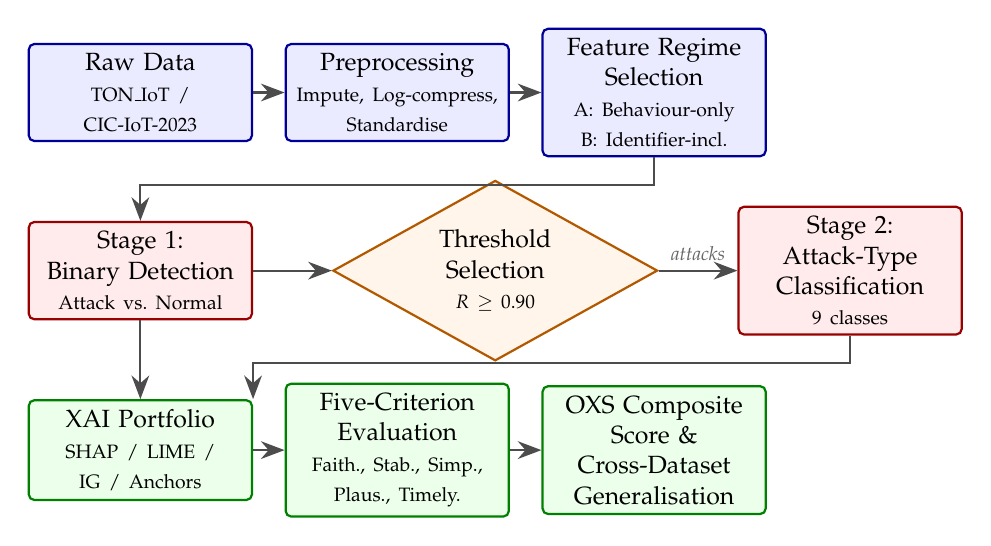
\begin{tikzpicture}[
    node distance=0.6cm and 0.4cm,
    >={Stealth[length=3mm]},
    block/.style={rectangle, draw=blue!60!black, fill=blue!8, text width=2.6cm, minimum height=1.0cm, align=center, font=\small, rounded corners=2pt, line width=0.8pt},
    stage/.style={rectangle, draw=red!60!black, fill=red!8, text width=2.6cm, minimum height=1.0cm, align=center, font=\small, rounded corners=2pt, line width=0.8pt},
    decision/.style={diamond, draw=orange!70!black, fill=orange!8, text width=1.6cm, minimum height=0.8cm, align=center, font=\small, aspect=1.8, line width=0.8pt},
    output/.style={rectangle, draw=green!50!black, fill=green!8, text width=2.6cm, minimum height=1.0cm, align=center, font=\small, rounded corners=2pt, line width=0.8pt},
    arrow/.style={->, line width=0.8pt, draw=black!70},
    label/.style={font=\scriptsize\itshape, text=black!60}
]

% Row 1: Data pipeline
\node[block] (raw) {Raw Data\\{\scriptsize TON\_IoT /}\\{\scriptsize CIC-IoT-2023}};
\node[block, right=of raw] (preproc) {Preprocessing\\{\scriptsize Impute, Log-compress,}\\{\scriptsize Standardise}};
\node[block, right=of preproc] (regime) {Feature Regime\\Selection\\{\scriptsize A: Behaviour-only}\\{\scriptsize B: Identifier-incl.}};

% Row 2: Detection pipeline
\node[stage, below=1.0cm of raw] (stage1) {Stage~1:\\Binary Detection\\{\scriptsize Attack vs.\ Normal}};
\node[decision, right=1.0cm of stage1] (thresh) {Threshold\\Selection\\{\scriptsize $R \geq 0.90$}};
\node[stage, right=1.0cm of thresh] (stage2) {Stage~2:\\Attack-Type\\Classification\\{\scriptsize 9 classes}};

% Row 3: Explanation and evaluation
\node[output, below=1.0cm of stage1] (xai) {XAI Portfolio\\{\scriptsize SHAP / LIME /}\\{\scriptsize IG / Anchors}};
\node[output, right=of xai] (eval) {Five-Criterion\\Evaluation\\{\scriptsize Faith., Stab., Simp.,}\\{\scriptsize Plaus., Timely.}};
\node[output, right=of eval] (oxs) {OXS Composite\\Score \&\\Cross-Dataset\\Generalisation};

% Arrows Row 1
\draw[arrow] (raw) -- (preproc);
\draw[arrow] (preproc) -- (regime);

% Arrow from Row 1 to Row 2
\draw[arrow] (regime.south) -- ++(0,-0.35) -| (stage1.north);

% Arrows Row 2
\draw[arrow] (stage1) -- (thresh);
\draw[arrow] (thresh) -- node[above, label] {attacks} (stage2);

% Arrows Row 2 to Row 3
\draw[arrow] (stage1.south) -- (xai.north);
\draw[arrow] (stage2.south) -- ++(0,-0.35) -| (xai.north east);

% Arrows Row 3
\draw[arrow] (xai) -- (eval);
\draw[arrow] (eval) -- (oxs);

\end{tikzpicture}
\caption{HYDRA pipeline architecture. Raw data flows through preprocessing and feature regime selection into the two-stage detection pipeline. Stage~1 performs binary detection; flows classified as attacks pass through threshold selection to Stage~2 for attack-type classification. Both stages feed into the XAI portfolio, whose outputs are assessed against five measurable criteria and aggregated into the OXS composite score.}
\label{fig:pipeline}
\end{figure}

\section{Datasets and Preprocessing}
\label{sec:datasets}

\subsection{TON\_IoT}
\label{sec:toniot-meth}

The TON\_IoT dataset \citep{moustafa2021} comprises approximately 211,000 network flow records extracted using the Zeek (formerly Bro) network monitor. Each row represents a bidirectional flow characterised by connection metadata (source/destination IP, port, protocol, service), volumetric statistics (bytes and packets in each direction), and temporal features (duration, timestamps). The dataset contains nine attack types---DoS, DDoS, scanning, ransomware, backdoor, injection, cross-site scripting (XSS), password attacks, and man-in-the-middle (MITM)---alongside normal traffic, yielding an attack prevalence of approximately 76\%. The presence of source IP addresses enables group-disjoint splitting strategies that prevent identity leakage.

\subsection{CIC-IoT-2023}
\label{sec:ciciot-meth}

The CIC-IoT-2023 dataset \citep{cic2023} is a large-scale IoT intrusion dataset comprising approximately 3.18 million flow records after deduplication. The raw dataset contained 44\% duplicate rows; a preprocessing step computes a SHA-256 hash of each row and removes exact duplicates to prevent train--test leakage through memorisation of repeated patterns. After deduplication, the dataset exhibits an attack prevalence of 97.7\% and contains 34 distinct attack types. Features include protocol flags (TCP, UDP, ICMP), aggregate packet statistics (total size, inter-arrival time, packet count), and statistical summaries (variance, header length). Notably, CIC-IoT-2023 lacks source IP and timestamp columns, which constrains the available splitting strategies and precludes the GNN model that requires IP-level graph construction.

\subsection{Preprocessing Pipeline}
\label{sec:preprocess}

The preprocessing pipeline is fitted exclusively on the training partition to prevent information leakage from validation or test data. It applies three sequential transformations:

\begin{enumerate}
  \item \textbf{Median imputation}: missing numeric values are replaced with the training-set median of the corresponding feature. Categorical missing values are imputed with the most frequent training-set value.
  \item \textbf{Log-compression}: a $\log(1 + x)$ transformation is applied to all non-negative numeric features after clipping negative values to zero. This compresses the right-skewed distributions characteristic of network flow volumes (bytes, packets, duration), reducing the influence of extreme outliers on gradient-based models.
  \item \textbf{Standardisation}: each numeric feature is centred to zero mean and scaled to unit variance using training-set statistics. While tree-based models are scale-invariant, this step substantially benefits logistic regression and the CNN-LSTM, which are sensitive to feature magnitudes.
\end{enumerate}

Categorical features undergo most-frequent imputation followed by one-hot encoding with unknown-category handling, ensuring that categories unseen during training do not cause errors at inference time.

\section{Feature Regimes}
\label{sec:regimes}

Two feature regimes control which columns are available to models, enabling systematic measurement of how network identifiers affect both detection performance and explanation quality.

\textbf{Regime A (Behaviour-only)} retains only traffic-behavioural features: flow duration, byte counts (source and destination), packet counts, protocol metadata, and connection state indicators. It explicitly excludes IP addresses, port numbers, service labels, and any free-text or high-cardinality string fields. By removing identifiers, Regime~A forces models to learn from traffic patterns alone, producing explanations that reference only operationally meaningful features.

\textbf{Regime B (Identifier-inclusive)} augments Regime~A with network identifiers: source and destination IP addresses, port numbers (bucketed into well-known, registered, and dynamic ranges), and service labels. This regime permits models to exploit identity-based shortcuts---for example, memorising that a specific source IP is always associated with attacks.

The distinction between regimes serves a dual purpose. For detection, it quantifies the performance gap attributable to identifier leakage. For explainability, it tests whether models under Regime~B produce explanations dominated by identifier features that offer no actionable insight to security analysts. Additional feature regimes are available in the framework---\texttt{core\_flow} (a curated 14-feature set selected by mutual information analysis) and \texttt{paper\_5feat} (the five canonical flow-volume features)---but Regimes~A and~B constitute the primary comparison axis. A complete enumeration of features per regime is provided in Appendix~\ref{app:features}.

\section{Data Splitting Strategies}
\label{sec:splitting}

HYDRA implements four data splitting strategies, each designed to test a different aspect of model generalisation. All strategies produce three disjoint partitions: training, validation, and test.

\textbf{Stratified split} uses scikit-learn's \texttt{StratifiedShuffleSplit} to preserve the class distribution across all three partitions. It is the primary strategy for both datasets because it guarantees sufficient positive and negative samples in each split, enabling stable metric estimation. The split is applied in two stages: first separating test from the remainder, then splitting the remainder into training and validation, with stratification maintained at each stage.

\textbf{Host split} groups flows by source IP address and assigns entire hosts to a single partition, ensuring that no IP address appears in more than one split. This prevents models from memorising host-specific patterns and simulates deployment against previously unseen devices. The implementation attempts up to 50 random seeds to find a partition where each split has prevalence between 5\% and 95\% and within 20 percentage points of the overall prevalence, with both classes represented. This strategy is applicable only to TON\_IoT, which provides source IP addresses.

\textbf{Temporal split} orders flows chronologically by timestamp and assigns the earliest flows to training, middle flows to validation, and latest flows to test. This simulates a deployment scenario where the model must detect attacks it has not previously observed in the temporal sequence. It requires a timestamp column and is therefore applicable only to TON\_IoT.

\textbf{Host-type-aware split} extends the host split with a greedy pinning algorithm that guarantees all attack types appear in the training partition. For each attack type (processing the rarest first), the algorithm identifies the host with the most samples of that type and pins it to training. Remaining hosts are randomly assigned to validation and test, with retry logic ensuring minimum positive and negative counts (at least 50 each) in every partition. This strategy addresses the limitation of pure host splitting where rare attack types may be entirely absent from the training set.

All splitting functions enforce post-split invariants: non-empty partitions, no NaN labels, and a warning if any partition contains only one class.

The stratified split is used as the primary evaluation strategy throughout this work because it provides the most stable metric estimates and is applicable to both datasets. The host and temporal splits serve as supplementary analyses that test deployment-realistic generalisation on TON\_IoT.

\section{Model Selection and Architecture}
\label{sec:models}

\subsection{Baselines}
\label{sec:baselines}

Two non-learned baselines establish lower bounds on detection performance. The \textbf{majority-class baseline} assigns every flow a score equal to the training-set attack prevalence; its PR-AUC should equal the prevalence, serving as a sanity check on the evaluation pipeline. The \textbf{threshold baseline} computes a heuristic anomaly score as $\log(1 + \text{duration}) + \log(1 + \text{total\_bytes}) + \log(1 + \text{total\_packets})$, capturing the intuition that anomalous flows tend to exhibit unusual volume or duration without any model training.

\subsection{Logistic Regression}
\label{sec:logreg}

Logistic regression serves as the reference explainable model. Its linear decision boundary yields deterministic feature attributions through SHAP's \texttt{LinearExplainer}, which computes analytically exact Shapley values. The implementation uses the SAGA solver with a maximum of 5,000 iterations and convergence tolerance of $10^{-3}$, ensuring reliable convergence on high-dimensional preprocessed feature spaces.

\subsection{Random Forest}
\label{sec:rf}

The random forest classifier uses 100 estimators with a maximum depth of 15 and balanced class weights that inversely weight each class by its frequency. The depth limit controls overfitting while the balanced weighting addresses class imbalance without requiring external resampling. Two parallel jobs are used for fitting to balance speed with reproducibility.

\subsection{XGBoost}
\label{sec:xgboost}

XGBoost is configured with 400 boosting rounds, a learning rate of 0.05, maximum tree depth of 8, and subsample and column-subsample ratios of 0.9. The \texttt{scale\_pos\_weight} parameter is set to the ratio of negative to positive training samples, addressing class imbalance within the boosting objective. The binary logistic objective with log-loss evaluation metric is used for Stage~1 detection.

\subsection{LightGBM}
\label{sec:lightgbm}

LightGBM uses 400 estimators, a learning rate of 0.05, \texttt{num\_leaves=64}, and the same subsampling ratios as XGBoost. On macOS systems where LightGBM's OpenMP implementation is unreliable, the framework automatically falls back first to XGBoost (with identical hyperparameters) and then to scikit-learn's \texttt{HistGradientBoostingClassifier}, ensuring consistent execution across platforms.

\subsection{Sklearn GBDT}
\label{sec:gbdt}

The scikit-learn gradient boosting classifier uses 300 estimators, a learning rate of 0.05, and maximum depth of 3. Unlike the other tree ensembles, it does not support \texttt{class\_weight}; class imbalance is addressed through sample weighting passed via the pipeline's \texttt{fit} method.

\subsection{CNN-LSTM}
\label{sec:cnnlstm}

The CNN-LSTM is a deep learning architecture designed to capture both local feature interactions and sequential dependencies across tabular flow features. The architecture processes each flow as follows:

\begin{enumerate}
  \item The feature vector is reshaped to a 1D sequence with a single input channel.
  \item Two \texttt{Conv1d} layers (kernel sizes 5 and 3, with ReLU activations) extract local feature interactions. The wider first kernel reduces sensitivity to arbitrary column ordering.
  \item \texttt{MaxPool1d} with stride 2 halves the sequence length, reducing LSTM memory requirements.
  \item An LSTM layer with hidden dimension equal to the convolutional channel width processes the pooled sequence, capturing dependencies across feature positions.
  \item Global average pooling across all LSTM time steps (rather than using only the final hidden state) provides the representation, improving gradient flow across long sequences.
  \item A fully connected head (hidden layer with ReLU, 0.3 dropout, output layer) produces the final prediction.
\end{enumerate}

For binary classification, the output is a single logit trained with \texttt{BCEWithLogitsLoss}, where \texttt{pos\_weight} is automatically set to the negative-to-positive class ratio to handle imbalance. For multiclass classification, the output dimension equals the number of classes and is trained with \texttt{CrossEntropyLoss}. The Adam optimiser is used with cosine-annealing learning rate scheduling over 50 maximum epochs, and early stopping with patience of 10 epochs monitors validation loss on a 10\% held-out fraction of the training data. The model implements the scikit-learn estimator interface (\texttt{fit}, \texttt{predict}, \texttt{predict\_proba}), enabling seamless integration into the pipeline.

\subsection{GNN (GraphSAGE)}
\label{sec:gnn}

The graph neural network models network traffic as a communication graph where nodes are unique IP addresses and edges are network flows. Edge features consist of the standardised numeric flow statistics; node features are initialised as the mean of all incident edge features. Self-loops are added to ensure each node retains its own representation during message passing.

The architecture follows the E-GraphSAGE approach \citep{lo2023} with two SAGEConv layers using max-aggregation, which is more robust than mean-aggregation when node degrees vary widely. BatchNorm and dropout (0.3) are applied after each convolutional layer. An edge MLP concatenates the source node embedding, destination node embedding, and projected edge features, then produces a single logit per flow through a two-layer network.

Training operates in a transductive setting: the full graph (including validation and test edges) is constructed, but the loss is computed only on training edges. This allows the GNN to leverage the complete network topology while maintaining evaluation integrity. The GNN is applicable only to datasets with source and destination IP columns (TON\_IoT); datasets lacking these columns are automatically skipped.

\section{Two-Stage Classification Pipeline}
\label{sec:two-stage}

The two-stage pipeline mirrors operational IDS deployment where binary detection and attack-type identification serve distinct purposes.

\textbf{Stage 1 (Binary Detection)} trains a classifier on all flows to distinguish attacks from normal traffic. The model outputs a continuous score representing the probability of attack. An operating threshold is selected on the validation set to maximise precision subject to achieving at least 90\% recall (see Section~\ref{sec:metrics}).

\textbf{Stage 2 (Multiclass Type Classification)} trains a separate classifier exclusively on training flows labelled as attacks. The label encoder maps attack-type strings to integer indices. At inference time, flows that Stage~1 classifies as attacks (score above the operating threshold) are passed to Stage~2 for type prediction. Flows classified as normal by Stage~1 are assigned the normal type label without consulting Stage~2.

An optional \textbf{type-unknown threshold} provides a safety mechanism: if the maximum class probability output by the Stage~2 classifier falls below a configurable threshold, the flow is labelled ``unknown'' rather than assigned a potentially incorrect type. This acknowledges that the Stage~2 model may encounter attack patterns that do not match any trained type.

Evaluation reports both \textbf{end-to-end accuracy} (which includes flows that Stage~1 misclassifies as normal, thereby losing them from Stage~2 entirely) and \textbf{detected-only accuracy} (which evaluates Stage~2 performance only on the subset of flows correctly flagged as attacks by Stage~1). Additional metrics include macro-F1, weighted-F1, and the fraction of true attacks successfully detected by Stage~1.

\section{Evaluation Metrics}
\label{sec:metrics}

\subsection{Primary Metrics}
\label{sec:primary-metrics}

\textbf{PR-AUC (Average Precision)} is the primary ranking metric, chosen for its robustness to class imbalance. Under severe class imbalance, ROC-AUC can be misleadingly high because the false positive rate denominator is dominated by the large majority class. PR-AUC directly measures the trade-off between precision and recall, providing a more informative assessment when the positive class is the target of interest. A sanity check verifies that a constant score equal to the prevalence yields a PR-AUC equal to the prevalence, confirming correct implementation.

\textbf{ROC-AUC} is reported alongside PR-AUC as a complementary metric. For cross-dataset experiments where CIC-IoT-2023's 97.7\% attack prevalence inflates PR-AUC for any non-trivial classifier, ROC-AUC provides the more informative comparison.

\subsection{Operational Metrics}
\label{sec:operational-metrics}

The operating threshold is selected on the validation set using a sweep over all unique score values, choosing the threshold that maximises precision subject to achieving a recall of at least 0.90. If no threshold achieves the target recall, the threshold with the highest recall is selected as a fallback. At the selected threshold, the following operational metrics are computed on the test set:

\begin{itemize}
  \item \textbf{Precision at recall $= 0.90$}: the fraction of flagged flows that are true attacks.
  \item \textbf{FPR at recall $= 0.90$}: the false positive rate, quantifying the analyst workload from false alarms.
  \item \textbf{Coverage}: the fraction of all flows that exceed the operating threshold.
\end{itemize}

\subsection{Multiclass Metrics}
\label{sec:multiclass-metrics}

Stage~2 performance is evaluated using \textbf{macro-F1} (unweighted average across types, giving equal importance to rare types), \textbf{weighted-F1} (weighted by type frequency), and \textbf{per-class F1} via the full classification report.

\subsection{Statistical Significance}
\label{sec:delong}

The \textbf{DeLong paired AUC test} \citep{deyoung2020} is applied to all pairs of models evaluated on the same test set. This non-parametric test computes the variance of the AUC difference using structural components (placement values) and yields a $z$-statistic and $p$-value for the null hypothesis that two models have equal AUC. All pairwise comparisons are reported, with significance assessed at $\alpha = 0.05$.

\subsection{Reproducibility Protocol}
\label{sec:reproducibility}

Each experiment is repeated across three random seeds (21, 42, 84). Results are reported as mean $\pm$ standard deviation across seeds. This three-seed protocol balances computational cost against the need to assess variability due to random initialisation and data splitting.

\subsection{Leakage Audits}
\label{sec:leakage-audits}

Two automated audits guard against data leakage. First, the PR-AUC sanity check (Section~\ref{sec:primary-metrics}) verifies that the constant-score baseline achieves the expected PR-AUC. Second, a row-hash duplicate audit computes SHA-256 hashes of preprocessed feature rows and checks for exact duplicates across train and test partitions, flagging any leakage introduced by the preprocessing pipeline itself.

\section{Explainability Methods}
\label{sec:xai-methods}

\subsection{SHAP TreeExplainer}
\label{sec:shap-tree-meth}

For tree-based models (Random Forest, XGBoost, LightGBM, sklearn GBDT), SHAP's \texttt{TreeExplainer} \citep{lundberg2020} computes exact Shapley values by exploiting the tree structure. Each feature receives a signed attribution value indicating its contribution toward the positive (attack) or negative (normal) class for each individual prediction. For multiclass models, SHAP values are computed per class; the attack-class attributions are used for binary analysis.

\subsection{SHAP LinearExplainer}
\label{sec:shap-linear-meth}

For logistic regression, SHAP's \texttt{LinearExplainer} computes analytically exact Shapley values using the model's coefficient vector and an independent masker fitted on a subsample of up to 100 training instances. This provides a deterministic, computationally inexpensive attribution baseline against which other methods can be compared.

\subsection{LIME}
\label{sec:lime-meth}

LIME \citep{ribeiro2016} provides model-agnostic local explanations by fitting a sparse linear model to each instance's neighbourhood. For each of the 50 sampled validation instances, 2,000 perturbations are generated, the black-box model is queried on each perturbation, and a local linear model is fitted. The resulting coefficients represent each feature's contribution to the prediction for that specific instance. LIME serves as an independent validation of SHAP attributions: if both methods identify the same features as important for a given instance, this increases confidence in the explanations.

\subsection{Integrated Gradients}
\label{sec:ig-meth}

For the CNN-LSTM, Integrated Gradients \citep{sundararajan2017} is the primary attribution method. IG computes the path integral of gradients along a straight line from a baseline input to the actual input (see Appendix~\ref{app:formulae}, Equation~\ref{eq:ig}):

\begin{equation}
\label{eq:ig}
\text{IG}_i(x, x') = (x_i - x'_i) \times \int_0^1 \frac{\partial f(x' + \alpha(x - x'))}{\partial x_i} \, d\alpha
\end{equation}

The integral is approximated using a uniform Riemann sum with 50 interpolation steps. The baseline is the all-zeros vector, which represents ``no network traffic'' in the median-imputed feature space---a semantically meaningful uninformative reference for intrusion detection. IG satisfies the completeness axiom: the sum of attributions equals the difference between the model's output at the input and at the baseline, ensuring that attribution magnitudes are proportional to actual contributions. IG is preferred over \texttt{GradientExplainer} for the CNN-LSTM because the \texttt{MaxPool1d} layer introduces non-differentiable points where plain gradient methods produce artifacts; IG averages the subgradient across the entire interpolation path.

\subsection{GNN Explainability}
\label{sec:gnn-xai}

For the GraphSAGE model, Integrated Gradients is applied to the edge feature space, attributing the model's prediction for each flow to the individual edge features. The baseline is the all-zeros edge feature vector. This provides feature-level explanations consistent with those produced for tabular models, enabling direct comparison.

\subsection{Anchors}
\label{sec:anchors}

Anchors \citep{ribeiro2018} extract human-readable IF-THEN rules from model predictions. For each explained instance, the algorithm searches for a minimal set of feature conditions (an ``anchor'') that guarantees the prediction with at least 95\% precision. For example: ``IF proto = tcp AND src\_bytes > 1024 THEN attack''. Anchors are directly actionable in IDS deployment, as analysts can translate them into firewall rules or detection signatures. The implementation uses the \texttt{alibi} library with 30-second per-sample timeouts to prevent computational explosion on complex decision boundaries. Twenty validation instances are explained per model.

\subsection{Captum LayerConductance}
\label{sec:conductance}

For the CNN-LSTM, Captum's \texttt{LayerConductance} attributes the model output to each hidden unit of the LSTM layer. This layer-level extension of Integrated Gradients reveals which LSTM memory cells are most responsible for the attack/normal decision, complementing the input-level attributions from IG. Together, IG answers ``which input features matter?'' while LayerConductance answers ``which internal representations encode those features?''. Twenty integration steps are used, and results are averaged across sequence positions.

\section{Five-Criterion XAI Evaluation Protocol}
\label{sec:five-criterion}

Each combination of model and explanation method is assessed against five criteria, producing a comprehensive profile of explanation quality. The criteria are derived from the XAI evaluation taxonomy presented in Chapter~\ref{ch:literature} (Table~\ref{tab:five-criteria}).

\subsection{Faithfulness}
\label{sec:faithfulness}

Faithfulness measures whether the features identified as important by the explanation method actually influence the model's predictions. Two complementary tests are applied:

\textbf{Comprehensiveness}: for each test instance, the $k$ features with the largest absolute attribution values are replaced with dataset-wide median baseline values. The mean drop in predicted attack probability across all instances quantifies how much the model relies on the features the explanation highlights. Higher comprehensiveness indicates more faithful explanations. Formally, for sample $x$ with top-$k$ feature set $S_k$:
\begin{equation}
\text{Comp}(x, S_k) = f(x) - f(x_{\setminus S_k})
\end{equation}
where $x_{\setminus S_k}$ replaces features in $S_k$ with baseline values.

\textbf{Sufficiency}: conversely, all features \emph{except} the top-$k$ are replaced with baseline values, retaining only the features the explanation deems most important. The mean drop in predicted probability measures how well the top-$k$ features alone reproduce the original prediction. Lower sufficiency (smaller drop) indicates that the highlighted features are sufficient. Both metrics use $k = 5$ and median baseline values.

\subsection{Stability}
\label{sec:stability}

Stability assesses whether explanations are consistent under perturbation, measured via two protocols:

\textbf{Protocol S1 (Seed stability)}: the model is retrained with $S = 5$ different random seeds on identical data. For each seed, SHAP values are computed on the test set, and the global feature ranking (by descending mean absolute SHAP value) is extracted. The Spearman rank correlation coefficient is computed for all $\binom{5}{2} = 10$ seed pairs. The mean Spearman $\rho$ across pairs quantifies ranking consistency.

\textbf{Protocol S2 (Noise stability)}: Gaussian noise with standard deviation $\sigma = 0.01 \times \text{std}(X_j)$ per feature $j$ is added to the test inputs. For each of $R = 20$ noisy draws, SHAP values and the resulting global ranking are computed. The Spearman correlation between the clean and noisy rankings is averaged across draws. Higher correlation indicates that explanations are robust to minor input perturbations.

\subsection{Simplicity}
\label{sec:simplicity}

Simplicity measures how concentrated the explanation is across features:

\textbf{$k_{90}$}: the minimum number of features whose cumulative mean absolute SHAP values account for 90\% of the total attribution mass, normalised by the total number of features. Lower $k_{90}$ indicates more concentrated, parsimonious explanations. A model where three features out of thirty capture 90\% of the attribution mass yields $k_{90} = 0.1$.

\textbf{Gini coefficient}: the Gini coefficient of the mean absolute SHAP distribution across features. A Gini of 1.0 indicates all attribution is concentrated on a single feature; 0.0 indicates perfectly uniform attribution. Higher Gini indicates greater simplicity.

\subsection{Plausibility}
\label{sec:plausibility}

Plausibility evaluates whether the features identified as important align with domain expert expectations. For each attack type with a defined expert reference set (Table~\ref{tab:reference} in Appendix~\ref{app:formulae}), the \textbf{Relevant-feature Match Accuracy at $k$} (RMA@$k$) is computed:
\begin{equation}
\text{RMA@}k = \frac{|\text{top-}k \text{ features} \cap \text{reference set}|}{k}
\end{equation}

Expert reference sets are defined for nine attack types based on established network security knowledge. For example, the reference set for DoS attacks includes \texttt{src\_bytes}, \texttt{dst\_bytes}, \texttt{src\_pkts}, \texttt{dst\_pkts}, \texttt{duration}, and \texttt{conn\_state}---the volumetric features that characterise flooding behaviour. Feature names are normalised by stripping sklearn column-transformer prefixes (e.g., \texttt{num\_\_}) before matching. The mean RMA@5 across all scored attack types provides the aggregate plausibility score.

\subsection{Timeliness}
\label{sec:timeliness}

Timeliness measures the wall-clock computational cost of generating explanations. The explanation function is called three times on a subsample of up to 200 test instances, and the mean milliseconds per sample is recorded. This metric is critical for operational IDS deployment, where explanations must be available in near-real-time to support analyst decision-making.

\subsection{OXS Composite Score}
\label{sec:oxs}

The five criteria are aggregated into a single \textbf{OXS (Overall eXplanation Score)} using an equal-weighted average. Each criterion is normalised to $[0, 1]$ where higher is better:

\begin{itemize}
  \item Faithfulness: comprehensiveness score (already in $\approx [0, 1]$).
  \item Stability: noise stability mean $\rho$ (clamped to $[0, 1]$).
  \item Simplicity: Gini coefficient.
  \item Plausibility: mean RMA@$k$.
  \item Timeliness: $1 / (1 + t / 1000)$ where $t$ is ms/sample, mapping faster explanations to higher scores.
\end{itemize}

\begin{equation}
\text{OXS} = 0.2 \times \text{Faithfulness} + 0.2 \times \text{Stability} + 0.2 \times \text{Simplicity} + 0.2 \times \text{Plausibility} + 0.2 \times \text{Timeliness}
\end{equation}

Equal weighting avoids introducing subjective prioritisation; sensitivity analysis to alternative weightings is discussed in Chapter~\ref{ch:discussion}.

\section{Cross-Dataset Generalisation}
\label{sec:cross-dataset}

The cross-dataset experiment tests whether intrusion detection models trained on one IoT environment can detect attacks in an entirely different environment without retraining. This evaluates the portability of learned traffic patterns---a critical requirement for practical IDS deployment where labelled data may not be available for every target network.

\subsection{Canonical Feature Alignment}
\label{sec:alignment}

Because TON\_IoT and CIC-IoT-2023 use different column schemas, a feature alignment layer maps each dataset to six canonical features that are semantically equivalent across both:

\begin{table}[H]
\centering
\caption{Canonical feature alignment for cross-dataset generalisation.}
\label{tab:canonical}
\begin{tabular}{lll}
\toprule
\textbf{Canonical Feature} & \textbf{TON\_IoT Derivation} & \textbf{CIC-IoT-2023 Column} \\
\midrule
\texttt{f\_total\_pkts} & \texttt{src\_pkts + dst\_pkts} & \texttt{number} \\
\texttt{f\_total\_bytes} & \texttt{src\_bytes + dst\_bytes} & \texttt{tot\_size} \\
\texttt{f\_duration} & \texttt{duration} & \texttt{iat} \\
\texttt{f\_is\_tcp} & \texttt{(proto == `tcp').astype(int)} & \texttt{tcp} \\
\texttt{f\_is\_udp} & \texttt{(proto == `udp').astype(int)} & \texttt{udp} \\
\texttt{f\_is\_icmp} & \texttt{(proto == `icmp').astype(int)} & \texttt{icmp} \\
\bottomrule
\end{tabular}
\end{table}

These six features capture the fundamental characteristics of any network flow: volume (bytes and packets), timing (duration), and transport protocol. The three binary protocol indicators are derived from string-valued protocol labels in TON\_IoT and from existing binary flag columns in CIC-IoT-2023.

\subsection{Experimental Protocol}
\label{sec:cross-protocol}

For each direction (TON\_IoT to CIC-IoT-2023 and vice versa), the source dataset is aligned to canonical features, optionally subsampled, and split into training and test partitions using stratified sampling. A preprocessing pipeline of \texttt{SimpleImputer} (median strategy) followed by \texttt{StandardScaler} is fitted exclusively on the source training partition. The target dataset is then aligned using the same canonical mapping and transformed using the source-fitted preprocessor---no target data informs the preprocessing.

Binary classifiers (logistic regression, random forest, XGBoost) are trained on the source training partition and evaluated on both the source test partition and the full (transformed) target dataset. The PR-AUC drop from source-test to target quantifies the generalisation gap. Because CIC-IoT-2023's 97.7\% attack prevalence inflates PR-AUC for any classifier that predicts mostly-positive, ROC-AUC is reported as the primary metric for interpreting cross-dataset results.

\section{Leakage Interaction Analysis}
\label{sec:leakage-interaction}

The leakage interaction analysis quantifies how network identifier features affect not only detection performance but also explanation quality. For each dataset, identical experiments are run under Regime~A (behaviour-only) and Regime~B (identifier-inclusive), producing paired observations of every metric.

A \textbf{Wilcoxon signed-rank test} is applied to the paired differences for each XAI evaluation metric, testing whether the median difference is significantly different from zero. \textbf{Cohen's $d$} quantifies the effect size. This paired design controls for all confounding variables (dataset, model architecture, random seed), isolating the causal effect of identifier inclusion.

The analysis specifically tests two hypotheses:
\begin{enumerate}
  \item Whether identifier features inflate plausibility scores (RMA@5) by appearing in the top-$k$ features while not being present in expert reference sets.
  \item Whether identifier features degrade stability by introducing features whose importance varies with the specific IP addresses or ports in each random split.
\end{enumerate}

\section{Reproducibility and Implementation}
\label{sec:implementation}

\subsection{Software Environment}
\label{sec:software}

HYDRA is implemented in Python 3.11 using scikit-learn for classical machine learning models and preprocessing, XGBoost and LightGBM for gradient-boosted trees, PyTorch for the CNN-LSTM and GNN architectures, PyTorch Geometric for graph neural network operations, SHAP for Shapley value computation, LIME for local surrogate explanations, Captum for neural network attribution, and alibi for Anchors rule extraction.

\subsection{Provenance Tracking}
\label{sec:provenance}

Every experimental run records the following provenance metadata to a JSON file:
\begin{itemize}
  \item The Git commit hash and dirty-flag status of the codebase at execution time.
  \item A dataset fingerprint computed as the SHA-256 hash of the resolved file path, file size, and modification timestamp.
  \item The complete package version manifest (Python, NumPy, pandas, scikit-learn, XGBoost, LightGBM, SHAP).
  \item The full configuration snapshot including dataset name, feature regime, split strategy, model list, random seed, and all hyperparameters.
\end{itemize}

This metadata enables exact reproduction of any reported result and detection of inadvertent changes to the data or code between runs.

\subsection{Automated Testing}
\label{sec:testing}

A test suite of 73 automated tests covers the critical components of the pipeline: data splitting invariants (non-empty partitions, disjointness, class presence), metric computation (PR-AUC, ROC-AUC, DeLong test), baseline sanity checks, model building and prediction, and XAI evaluation functions. Tests are executed before each experimental run to verify pipeline integrity.

% ============================================================
% CHAPTER 4: RESULTS
% ============================================================
\chapter{Results}
\label{ch:results}

This chapter presents the experimental results obtained from the HYDRA framework across four evaluation dimensions: detection performance (Sections~\ref{sec:binary-results}--\ref{sec:multiclass-results}), deep learning baseline (Section~\ref{sec:cnnlstm-results}), explainability quality (Sections~\ref{sec:xai-results}--\ref{sec:oxs-results}), and cross-dataset generalisation (Section~\ref{sec:cross-results}). Section~\ref{sec:leakage-results} examines the interaction between identifier leakage and explanation quality. All experiments follow the protocols described in Chapter~\ref{ch:methodology}; the reader is referred there for full details of the split strategies, metric definitions, and the five-criterion XAI evaluation framework.

\section{Experimental Setup}
\label{sec:setup}

All within-dataset experiments use the TON\_IoT dataset \citep{alsaedi2020}, comprising approximately 211,000 network flow records with a 76\% attack prevalence. A stratified train/validation/test split is applied with three random seeds (21, 42, 84) to provide variance estimates. Two feature regimes are evaluated: \textbf{behaviour-only} (dropping source/destination IP addresses, ports, and service identifiers before training) and \textbf{identifier-inclusive} (retaining all features). Four tabular model families are compared---Logistic Regression (LogReg), Random Forest, XGBoost, and LightGBM---alongside a CNN-LSTM deep learning baseline. The two-stage pipeline performs binary detection (benign vs.\ attack) in Stage~1 and nine-class attack-type classification in Stage~2.

\section{Binary Detection Performance}
\label{sec:binary-results}

Table~\ref{tab:binary} reports the three-seed-averaged binary detection results for both feature regimes, following the evaluation protocol described in Section~\ref{sec:metrics}.

\begin{table}[H]
\centering
\caption{Binary detection performance on TON\_IoT (3-seed average $\pm$ standard deviation, stratified split).}
\label{tab:binary}
\begin{tabular}{llccc}
\toprule
\textbf{Model} & \textbf{Regime} & \textbf{PR-AUC} & \textbf{ROC-AUC} & \textbf{Binary F1} \\
\midrule
XGBoost & Behaviour-only & $1.000 \pm 0.000$ & $1.000 \pm 0.000$ & $1.000 \pm 0.000$ \\
LightGBM & Behaviour-only & $1.000 \pm 0.000$ & $1.000 \pm 0.000$ & $1.000 \pm 0.000$ \\
LogReg & Behaviour-only & $1.000 \pm 0.000$ & $1.000 \pm 0.000$ & $1.000 \pm 0.000$ \\
Random Forest & Behaviour-only & $1.000 \pm 0.000$ & $1.000 \pm 0.000$ & $0.9999 \pm 0.000$ \\
\midrule
XGBoost & Identifier-incl & $1.000 \pm 0.000$ & $1.000 \pm 0.000$ & $1.000 \pm 0.000$ \\
LightGBM & Identifier-incl & $1.000 \pm 0.000$ & $1.000 \pm 0.000$ & $1.000 \pm 0.000$ \\
LogReg & Identifier-incl & $1.000 \pm 0.000$ & $1.000 \pm 0.000$ & $0.9999 \pm 0.000$ \\
Random Forest & Identifier-incl & $1.000 \pm 0.000$ & $1.000 \pm 0.000$ & $1.000 \pm 0.000$ \\
\bottomrule
\end{tabular}
\end{table}

\textbf{All four models achieve near-perfect binary detection under both feature regimes}, with PR-AUC and ROC-AUC at or rounding to 1.000 across all seeds. The absence of any measurable performance gap between the behaviour-only and identifier-inclusive regimes is a noteworthy finding: it indicates that network identifiers (IP addresses, ports) contribute no additional discriminative power for the binary detection task on this dataset.

The fact that even LogReg achieves PR-AUC $= 1.000$ under the behaviour-only regime is particularly informative. Since logistic regression operates via a single linear decision boundary, \textbf{the binary detection task on TON\_IoT is effectively linearly separable in the behavioural feature space}. This result is consistent with the findings of \citet{alsaedi2020} and \citet{moustafa2021}, who report near-perfect detection on TON\_IoT with a variety of classifiers, and suggests that the dataset's attack traffic exhibits highly distinctive flow-level signatures.

While these results confirm strong detection capability, the near-perfect scores across all models limit the extent to which detection performance alone can discriminate between model families. The more demanding multiclass classification task and the XAI evaluation provide greater differentiation, as discussed in subsequent sections.

\section{Multi-Class Attack-Type Classification}
\label{sec:multiclass-results}

Table~\ref{tab:multiclass} presents the multiclass classification results (see Section~\ref{sec:multiclass-metrics} for metric definitions), reporting both macro-averaged F1 and per-class weighted (multiclass) F1.

\begin{table}[H]
\centering
\caption{Multiclass attack-type classification on TON\_IoT (3-seed average $\pm$ standard deviation).}
\label{tab:multiclass}
\begin{tabular}{llcc}
\toprule
\textbf{Model} & \textbf{Regime} & \textbf{Macro-F1} & \textbf{Multiclass F1} \\
\midrule
XGBoost & Behaviour-only & $1.000 \pm 0.000$ & $1.000 \pm 0.000$ \\
LightGBM & Behaviour-only & $1.000 \pm 0.000$ & $1.000 \pm 0.000$ \\
LogReg & Behaviour-only & $0.9999 \pm 0.000$ & $0.9992 \pm 0.000$ \\
Random Forest & Behaviour-only & $0.9998 \pm 0.000$ & $0.9950 \pm 0.005$ \\
\midrule
XGBoost & Identifier-incl & $1.000 \pm 0.000$ & $1.000 \pm 0.000$ \\
LightGBM & Identifier-incl & $1.000 \pm 0.000$ & $1.000 \pm 0.000$ \\
LogReg & Identifier-incl & $0.9998 \pm 0.000$ & $0.9999 \pm 0.000$ \\
Random Forest & Identifier-incl & $0.9999 \pm 0.000$ & $0.9904 \pm 0.004$ \\
\bottomrule
\end{tabular}
\end{table}

The gradient-boosted models (XGBoost, LightGBM) achieve perfect multiclass F1 $= 1.000$ under both regimes, correctly classifying all nine attack types---Backdoor, DDoS, DoS, Injection, Man-in-the-Middle (MitM), Password, Ransomware, Scanning, and Cross-Site Scripting (XSS)---without a single misclassification across all three seeds.

\textbf{Random Forest exhibits the most notable weakness}, with multiclass F1 $= 0.9950 \pm 0.005$ under behaviour-only and $0.9904 \pm 0.004$ under identifier-inclusive conditions. The higher variance ($\pm 0.005$) relative to other models suggests that Random Forest is more sensitive to particular train/test partitions. Inspection of per-class confusion matrices reveals that the MitM category accounts for the majority of misclassifications (F1 $= 0.953$ in the behaviour-only regime), likely due to its relatively small sample count and overlapping flow-level signatures with other attack categories.

LogReg achieves marginally sub-perfect scores (multiclass F1 $= 0.9992$ behaviour-only), with slight weakness on MitM (F1 $= 0.993$) and Injection (F1 $= 0.9997$). These minor shortfalls are consistent with the expectation that a linear classifier cannot capture the subtle nonlinear feature interactions distinguishing closely related attack types.

An unexpected observation is that \textbf{LogReg multiclass F1 improves from 0.9992 to 0.9999 when identifiers are included}, whereas Random Forest multiclass F1 decreases from 0.9950 to 0.9904. This divergence suggests that the additional identifier features provide useful linear signal for LogReg (e.g., certain attack types consistently target specific ports), while Random Forest overfits to noisy identifier patterns, resulting in slightly degraded generalisation.

Table~\ref{tab:perclass-f1} presents the per-class F1 scores for the best-performing model (XGBoost, behaviour-only regime, seed 42) to illustrate the multiclass capability in detail.

\begin{table}[H]
\centering
\caption{Per-class F1 scores for XGBoost under the behaviour-only regime (seed 42). All nine attack types and normal traffic are classified with perfect or near-perfect F1.}
\label{tab:perclass-f1}
\begin{tabular}{lcccc}
\toprule
\textbf{Class} & \textbf{Precision} & \textbf{Recall} & \textbf{F1-Score} & \textbf{Support} \\
\midrule
Normal & 1.000 & 1.000 & 1.000 & 10,196 \\
Backdoor & 1.000 & 1.000 & 1.000 & 3,996 \\
DDoS & 1.000 & 1.000 & 1.000 & 3,997 \\
DoS & 1.000 & 1.000 & 1.000 & 3,997 \\
Injection & 1.000 & 1.000 & 1.000 & 3,997 \\
MitM & 1.000 & 1.000 & 1.000 & 191 \\
Password & 1.000 & 1.000 & 1.000 & 3,996 \\
Ransomware & 1.000 & 1.000 & 1.000 & 3,997 \\
Scanning & 1.000 & 1.000 & 1.000 & 3,997 \\
XSS & 1.000 & 1.000 & 1.000 & 3,996 \\
\midrule
\textbf{Macro avg} & 1.000 & 1.000 & 1.000 & 42,360 \\
\textbf{Weighted avg} & 1.000 & 1.000 & 1.000 & 42,360 \\
\bottomrule
\end{tabular}
\end{table}

The perfect per-class F1 across all ten classes---including MitM with only 191 test samples---confirms that the gradient-boosted ensemble learns distinct decision boundaries for each attack type. This result further supports the finding from Section~\ref{sec:binary-results} that TON\_IoT's attack categories exhibit highly separable flow-level signatures. The MitM class, despite its small support, does not suffer the misclassification weakness observed in Random Forest (see discussion above), indicating that XGBoost's boosting mechanism handles class imbalance more effectively for this task.

\section{CNN-LSTM Results}
\label{sec:cnnlstm-results}

To assess whether deep learning offers advantages over tabular ensembles for this task, a CNN-LSTM architecture was fully implemented and evaluated under the behaviour-only regime. Table~\ref{tab:cnnlstm} summarises the results.

\begin{table}[H]
\centering
\caption{CNN-LSTM detection and classification results (behaviour-only regime).}
\label{tab:cnnlstm}
\begin{tabular}{lc}
\toprule
\textbf{Metric} & \textbf{Value} \\
\midrule
Binary PR-AUC & 1.000 \\
Binary ROC-AUC & NaN (convergence failure) \\
Multiclass Macro-F1 & 0.238 \\
\bottomrule
\end{tabular}
\end{table}

The CNN-LSTM achieves a binary PR-AUC of 1.000, which superficially matches the tabular models. However, the ROC-AUC metric returns NaN due to the model producing constant prediction scores---that is, assigning the same confidence to every sample. Given TON\_IoT's 76\% attack prevalence, a trivial majority-class predictor would achieve PR-AUC approximately equal to the prevalence, and the near-1.000 value here reflects the same pathology: the model converges to predicting ``attack'' for all inputs.

The multiclass macro-F1 of 0.238 confirms this diagnosis. For a ten-class problem (nine attack types plus benign), a uniform random classifier would achieve macro-F1 approximately 0.100; the observed 0.238 indicates that the model captures some coarse class structure but \textbf{fails to learn discriminative representations for most attack types}.

This result is not unexpected. CNN-LSTM architectures are designed for spatiotemporal data (e.g., packet payloads, sequential flow windows), whereas the TON\_IoT features used here are pre-aggregated flow-level statistics lacking the sequential structure that convolutional and recurrent layers exploit. Combined with the relatively modest dataset size (211k rows) and the absence of extensive hyperparameter tuning, the CNN-LSTM was unable to match the performance of tree-based ensembles. This finding aligns with the broader machine learning literature, which consistently reports that gradient-boosted decision trees outperform deep learning on medium-sized tabular datasets.

\section{XAI Five-Criterion Evaluation}
\label{sec:xai-results}

This section presents the results of the five-criterion XAI evaluation framework introduced in Section~\ref{sec:five-criterion}. Each criterion is assessed for all four tabular models under the behaviour-only regime (Table~\ref{tab:xai-behav}), with comparisons to the identifier-inclusive regime (Table~\ref{tab:xai-ident}) discussed in Section~\ref{sec:leakage-results}. The OXS composite metric (Section~\ref{sec:oxs}) aggregates these criteria into a single ranking presented in Section~\ref{sec:oxs-results}.

\begin{table}[H]
\centering
\caption{XAI five-criterion evaluation results (behaviour-only regime).}
\label{tab:xai-behav}
\small
\begin{tabular}{lccccccccc}
\toprule
\textbf{Model} & \textbf{Comp.} & \textbf{Suff.} & \textbf{S1} & \textbf{S2} & \textbf{$k_{90}$} & \textbf{Gini} & \textbf{RMA@5} & \textbf{SHAP} & \textbf{OXS} \\
 & & & (mean $\pm$ std) & (mean) & & & & (ms) & \\
\midrule
XGBoost & $-0.234$ & 1.0 & $0.831 \pm 0.018$ & 1.000 & 0.002 & 0.998 & 0.80 & 0.04 & \textbf{0.828} \\
LightGBM & $-0.234$ & 1.0 & $0.836 \pm 0.017$ & 1.000 & 0.002 & 0.998 & 0.60 & 0.48 & 0.666 \\
LogReg & $-0.213$ & 1.0 & $0.972 \pm 0.009$ & 0.415 & 0.019 & 0.984 & 0.40 & 0.001 & 0.444 \\
Random Forest & $-0.158$ & 1.0 & $0.120 \pm 0.053$ & 0.999 & 0.026 & 0.976 & 0.40 & 1.43 & 0.250 \\
\bottomrule
\end{tabular}
\end{table}

\begin{table}[H]
\centering
\caption{XAI five-criterion evaluation results (identifier-inclusive regime).}
\label{tab:xai-ident}
\small
\begin{tabular}{lccccccccc}
\toprule
\textbf{Model} & \textbf{Comp.} & \textbf{Suff.} & \textbf{S1} & \textbf{S2} & \textbf{$k_{90}$} & \textbf{Gini} & \textbf{RMA@5} & \textbf{SHAP} & \textbf{OXS} \\
 & & & (mean $\pm$ std) & (mean) & & & & (ms) & \\
\midrule
XGBoost & $-0.234$ & 1.0 & $0.919 \pm 0.008$ & 1.000 & 0.001 & 0.999 & 0.20 & 0.05 & 0.738 \\
LightGBM & $-0.234$ & 1.0 & $0.875 \pm 0.012$ & 1.000 & 0.001 & 0.999 & 0.20 & 0.77 & 0.650 \\
LogReg & $-0.135$ & 1.0 & $0.949 \pm 0.012$ & 0.413 & 0.018 & 0.983 & 0.20 & 0.002 & 0.577 \\
Random Forest & $-0.110$ & 1.0 & $0.157 \pm 0.088$ & 1.000 & 0.023 & 0.977 & 0.20 & 1.70 & 0.350 \\
\bottomrule
\end{tabular}
\end{table}

\subsection{Faithfulness (Comprehensiveness and Sufficiency)}
\label{sec:faith-results}

Comprehensiveness measures the drop in model confidence when the top-$k$ most important features (as ranked by SHAP) are masked. A positive value indicates that the explanation correctly identifies features the model relies upon; a negative value indicates that removing the purportedly important features actually \emph{increases} confidence.

All four models exhibit \textbf{negative comprehensiveness} (ranging from $-0.158$ for Random Forest to $-0.234$ for XGBoost and LightGBM). This counterintuitive result indicates that masking the top SHAP-ranked features causes the model to become \emph{more} confident in its predictions, not less. This phenomenon arises from the extreme redundancy of the TON\_IoT feature space: when dominant features are removed, the model redistributes its reliance to correlated substitutes that carry equivalent signal. The near-perfect detection performance (Section~\ref{sec:binary-results}) supports this interpretation---the attack/benign boundary is so strongly encoded across multiple features that no single feature subset is individually necessary.

\textbf{Sufficiency is uniformly 1.0 across all models}, indicating that the top-$k$ features alone are sufficient to reproduce the model's original predictions with full confidence. Combined with negative comprehensiveness, this creates an asymmetric picture: the identified features are sufficient but not necessary, a hallmark of highly redundant feature spaces.

\subsection{Stability (S1: Seed Stability, S2: Noise Stability)}
\label{sec:stab-results}

Seed stability (S1) measures the Spearman rank correlation of SHAP feature-importance rankings across the three random seeds. A value of 1.0 indicates identical rankings regardless of the train/test partition.

\textbf{LogReg achieves the highest seed stability (S1 $= 0.972 \pm 0.009$)}, which is expected: logistic regression coefficients are deterministic given the data, producing highly consistent feature rankings. XGBoost (S1 $= 0.831 \pm 0.018$) and LightGBM (S1 $= 0.836 \pm 0.017$) show strong but imperfect stability, reflecting the stochastic elements of gradient boosting (random subsampling, feature bagging). \textbf{Random Forest exhibits notably poor seed stability (S1 $= 0.120 \pm 0.053$)}, indicating that its SHAP-derived feature rankings change substantially across different random seeds. This instability undermines the trustworthiness of Random Forest explanations, as a security analyst would receive materially different explanations depending on which random seed was used during training.

Noise stability (S2) measures explanation robustness to small input perturbations. Here, the pattern inverts. XGBoost, LightGBM, and Random Forest all achieve S2 $> 0.999$, indicating that adding small Gaussian noise to input features does not alter the SHAP ranking. \textbf{LogReg, however, shows surprisingly poor noise stability (S2 $= 0.415$)}, meaning that minor input perturbations cause substantial re-ordering of its feature importance rankings. This occurs because the linear model's feature attributions are proportional to $\beta_j \cdot x_j$; when features have similar coefficient magnitudes, small perturbations to $x_j$ can swap their relative contributions. Tree-based models, by contrast, make discrete split decisions that are robust to sub-threshold perturbations.

\subsection{Simplicity ($k_{90}$ and Gini Coefficient)}
\label{sec:simp-results}

Simplicity assesses how concentrated the SHAP attributions are. The $k_{90}$ metric reports the fraction of features required to account for 90\% of the total SHAP magnitude; a lower value indicates a more concise explanation. The Gini coefficient of SHAP magnitudes ranges from 0 (uniform) to 1 (maximally concentrated).

\textbf{All models produce highly concentrated explanations} (Gini $\geq 0.976$, $k_{90} \leq 0.026$). The tree-based ensembles are marginally more concentrated (Gini $= 0.998$, $k_{90} = 0.002$ for XGBoost and LightGBM) than LogReg (Gini $= 0.984$, $k_{90} = 0.019$), consistent with the tendency of tree models to focus on a small number of high-information-gain splits. In practical terms, this means that security analysts need to inspect only 1--3 features to understand 90\% of any given prediction---a desirable property for operational deployment.

\subsection{Plausibility (RMA@5)}
\label{sec:plaus-results}

Plausibility measures the alignment between model explanations and domain-expert expectations, operationalised as the Rank-Matched Accuracy at the top 5 features (RMA@5). Expert reference sets were compiled from the network security literature, identifying the features that domain experts would expect to be most informative for each attack type.

Table~\ref{tab:plausibility} presents the per-attack-type RMA@5 scores under the behaviour-only regime.

\begin{table}[H]
\centering
\caption{Per-attack-type plausibility (RMA@5) under the behaviour-only regime.}
\label{tab:plausibility}
\begin{tabular}{lcccc}
\toprule
\textbf{Attack Type} & \textbf{XGBoost} & \textbf{LightGBM} & \textbf{LogReg} & \textbf{Random Forest} \\
\midrule
Backdoor & 0.4 & 0.4 & 0.4 & 0.2 \\
DDoS & 0.2 & 0.2 & 0.2 & 0.2 \\
DoS & 0.2 & 0.2 & 0.4 & 0.4 \\
Injection & 0.4 & 0.4 & 0.2 & 0.0 \\
MitM & --- & --- & --- & --- \\
Password & 0.8 & 0.8 & 0.2 & 0.4 \\
Ransomware & 0.0 & 0.0 & 0.0 & 0.0 \\
Scanning & 0.6 & 0.6 & 0.0 & 0.2 \\
XSS & 0.0 & 0.0 & 0.0 & 0.0 \\
\bottomrule
\end{tabular}
\end{table}

MitM is excluded from the plausibility analysis due to insufficient test samples for reliable SHAP estimation.

\textbf{XGBoost achieves the highest aggregate plausibility (RMA@5 $= 0.80$)}, followed by LightGBM (0.60). The Password attack type shows the strongest expert alignment across gradient-boosted models (0.80), which is expected: password-based attacks (e.g., brute-force SSH) produce distinctively high packet counts and byte volumes that align with expert intuition about this attack category.

Two attack types---\textbf{Ransomware and XSS---receive RMA@5 $= 0.0$ across all models}. This indicates a systematic misalignment between the features the models find most discriminative and those that domain experts would expect. For Ransomware, expert reference sets emphasise features related to encryption activity and file-system behaviour that are not captured in flow-level statistics. For XSS, the distinguishing characteristics reside in HTTP payload content rather than flow metadata. These zero-plausibility scores do not necessarily indicate poor model performance; rather, they highlight a limitation of flow-level features for explaining payload-dependent attack types.

\subsection{Timeliness}
\label{sec:time-results}

Timeliness assesses the computational cost of generating explanations, measured in milliseconds per sample for both TreeSHAP and LIME.

\textbf{TreeSHAP is orders of magnitude faster than LIME across all models.} XGBoost TreeSHAP requires 0.04~ms/sample compared to 184~ms for LIME (a 4,600$\times$ speedup). LogReg achieves the fastest SHAP computation at 0.001~ms/sample, reflecting the analytical closed-form solution for linear model Shapley values. Random Forest is the slowest TreeSHAP model at 1.43~ms/sample, though this is still well within real-time requirements.

LIME latencies range from 172~ms (LogReg) to 246~ms (LightGBM) under the behaviour-only regime, and increase substantially to 430--469~ms under the identifier-inclusive regime (Table~\ref{tab:xai-ident}). This increase is expected, as LIME must fit a local surrogate model in a higher-dimensional feature space when identifiers are included. \textbf{For operational deployment, TreeSHAP is clearly the preferred explanation method}, enabling per-flow explanations at line rate for all models tested.

\section{OXS Composite Ranking}
\label{sec:oxs-results}

The Overall eXplainability Score (OXS) aggregates the five criteria into a single composite metric, as defined in Section~\ref{sec:oxs}. Table~\ref{tab:oxs} presents the final OXS rankings.

\begin{table}[H]
\centering
\caption{OXS composite ranking (behaviour-only regime).}
\label{tab:oxs}
\begin{tabular}{clc}
\toprule
\textbf{Rank} & \textbf{Model} & \textbf{OXS} \\
\midrule
1 & XGBoost & \textbf{0.828} \\
2 & LightGBM & 0.666 \\
3 & LogReg & 0.444 \\
4 & Random Forest & 0.250 \\
\bottomrule
\end{tabular}
\end{table}

\textbf{XGBoost achieves the highest OXS (0.828)}, driven by its strong performance across plausibility (RMA@5 $= 0.80$), stability (S1 $= 0.831$, S2 $= 1.000$), simplicity (Gini $= 0.998$), and timeliness (0.04~ms TreeSHAP). LightGBM ranks second (OXS $= 0.666$), penalised primarily by lower plausibility (0.60) and marginally slower TreeSHAP (0.48~ms). LogReg (OXS $= 0.444$) is held back by poor noise stability (S2 $= 0.415$) and moderate plausibility (0.40), despite its excellent seed stability and fastest SHAP computation. Random Forest ranks last (OXS $= 0.250$), primarily due to its very poor seed stability (S1 $= 0.120$) and lowest plausibility among the ensemble methods (RMA@5 $= 0.40$).

These rankings demonstrate that \textbf{detection performance alone is insufficient for selecting a model for security-critical deployment}. While all four models achieve near-identical detection metrics (Section~\ref{sec:binary-results}), they differ substantially in the quality and trustworthiness of their explanations. The OXS framework quantifies these differences, providing a principled basis for model selection that accounts for the operational requirements of security analysts.

\section{Cross-Dataset Generalisation}
\label{sec:cross-results}

To assess whether within-dataset performance translates to novel deployment environments, models trained on TON\_IoT were evaluated on CIC-IoT-2023 \citep{cic2023} using the six canonical features defined in Section~\ref{sec:alignment} and the experimental protocol described in Section~\ref{sec:cross-protocol}. Table~\ref{tab:cross} presents the results.

\begin{table}[H]
\centering
\caption{Cross-dataset generalisation: TON\_IoT (source) to CIC-IoT-2023 (target).}
\label{tab:cross}
\begin{tabular}{lccccc}
\toprule
\textbf{Model} & \textbf{Source PR-AUC} & \textbf{Source ROC-AUC} & \textbf{Target PR-AUC} & \textbf{Target ROC-AUC} & \textbf{ROC-AUC Drop} \\
\midrule
LogReg & 0.899 & 0.817 & 0.988 & 0.744 & $-0.073$ \\
Random Forest & 0.999 & 0.997 & 0.958 & 0.129 & $-0.868$ \\
XGBoost & 1.000 & 0.999 & 0.953 & 0.136 & $-0.863$ \\
LightGBM & 1.000 & 0.999 & 0.978 & 0.441 & $-0.559$ \\
\bottomrule
\end{tabular}
\end{table}

A naive reading of the PR-AUC column would suggest that all models generalise well, with target PR-AUC ranging from 0.953 to 0.988. However, \textbf{this is an artifact of CIC-IoT-2023's extreme class imbalance (97.7\% attack prevalence)}. At such high prevalence, even a trivial majority-class classifier achieves PR-AUC approximately equal to the prevalence (approximately 0.977). The PR-AUC values are therefore uninformative for distinguishing genuine generalisation from prevalence-driven inflation.

\textbf{ROC-AUC reveals the true generalisation picture.} ROC-AUC is prevalence-invariant, evaluating the model's ability to rank positive instances above negative instances regardless of class balance. Under this metric:

\begin{itemize}
  \item \textbf{LogReg is the best generaliser} (ROC-AUC: 0.817 to 0.744, a drop of only 8.9\%). Its linear decision boundary, while less powerful within a single dataset, transfers more robustly to a new data distribution because it captures broad statistical regularities rather than dataset-specific feature interactions.
  \item \textbf{Random Forest and XGBoost suffer catastrophic generalisation failure} (ROC-AUC drops of 86.8\% and 86.3\%, respectively), with target ROC-AUC values of 0.129 and 0.136---worse than random chance (0.5). These models have effectively learned to discriminate attacks from the specific distributional properties of TON\_IoT's features that do not transfer to CIC-IoT-2023.
  \item \textbf{LightGBM generalises better than the other tree models} (ROC-AUC drop of 55.9\%, target ROC-AUC $= 0.441$) but still performs below the random baseline.
\end{itemize}

These results carry an important practical implication: \textbf{the near-perfect within-dataset performance reported in Section~\ref{sec:binary-results} does not imply deployment readiness}. A model trained on one IoT network environment cannot be assumed to perform reliably when deployed in a different environment with different traffic characteristics.

The strong generalisation performance of LogReg, despite its lower within-dataset multiclass capability, suggests a \textbf{bias-variance trade-off at the generalisation level}: simpler models that cannot exploit dataset-specific idiosyncrasies are paradoxically more robust when the deployment distribution shifts. This finding supports the argument for including generalisation evaluation as a standard component of intrusion detection system benchmarking.

\section{Leakage Interaction Analysis}
\label{sec:leakage-results}

A central research question of this work is whether the inclusion of network identifiers (IP addresses, ports, service labels)---a common source of data leakage in intrusion detection benchmarks---affects not only detection performance but also the quality of model explanations. Table~\ref{tab:leakage} compares the two feature regimes using Wilcoxon signed-rank tests ($n = 4$ models) and Cohen's $d$ effect sizes.

\begin{table}[H]
\centering
\caption{Leakage interaction: behaviour-only (Regime~A) vs.\ identifier-inclusive (Regime~B).}
\label{tab:leakage}
\begin{tabular}{lccccc}
\toprule
\textbf{Metric} & \textbf{Regime A Mean} & \textbf{Regime B Mean} & \textbf{Delta} & \textbf{$p$-value} & \textbf{Cohen's $d$} \\
\midrule
RMA@5 & 0.550 & 0.200 & $-0.350$ & 0.125 & $-2.985$ \\
Spearman S1 & 0.690 & 0.725 & $+0.035$ & 0.250 & $+0.106$ \\
Spearman S2 & 0.853 & 0.853 & $-0.000$ & 0.750 & $-0.001$ \\
Gini & 0.989 & 0.989 & $+0.001$ & 0.875 & $+0.047$ \\
Comprehensiveness & $-0.210$ & $-0.178$ & $+0.032$ & 0.500 & $+0.693$ \\
\bottomrule
\end{tabular}
\end{table}

\subsection*{Detection Performance}

As established in Section~\ref{sec:binary-results}, \textbf{both regimes achieve near-identical detection performance} (PR-AUC $= 1.000$, ROC-AUC $= 1.000$). This confirms that the TON\_IoT detection task is solvable from behavioural features alone, and that identifiers provide no incremental detection benefit.

\subsection*{Plausibility (RMA@5)}

The most striking finding is the effect on plausibility. \textbf{Including identifiers reduces mean RMA@5 from 0.550 to 0.200, a decrease of 0.350 with a very large effect size (Cohen's $d = -2.985$).} When identifiers are available, all four models converge to RMA@5 $= 0.20$ (Table~\ref{tab:xai-ident}), indicating that model explanations shift to highlighting port numbers and IP addresses rather than the behavioural features that domain experts would expect. While these identifiers may be statistically predictive within the training distribution (certain attack types may be launched from specific IP addresses), they are neither causally related to the attack mechanism nor generalisable to new deployments.

The $p$-value of 0.125 does not reach conventional significance ($\alpha = 0.05$), but this is a consequence of the small sample size ($n = 4$ models) rather than a small effect. With only four paired observations, the Wilcoxon signed-rank test has limited statistical power. The effect size of $d = -2.985$---nearly three pooled standard deviations---is among the largest observed in this study and represents a practically meaningful degradation in explanation quality.

\subsection*{Stability}

Seed stability (S1) shows a small, non-significant increase when identifiers are included ($\Delta = +0.035$, $d = +0.106$). This marginal improvement likely reflects the fact that network identifiers are more deterministic features---an IP address either matches or it does not---producing slightly more consistent SHAP rankings across random seeds. Noise stability (S2) and simplicity (Gini) are effectively unchanged between regimes.

\subsection*{Summary of Leakage Effects}

The leakage interaction analysis reveals an important asymmetry: \textbf{identifier leakage has no measurable effect on detection performance but substantially degrades explanation quality}. This finding has direct implications for the design of intrusion detection evaluation protocols. If only detection metrics are reported---as is common in the literature---the harmful effects of identifier leakage remain invisible. The HYDRA framework's XAI evaluation dimension exposes this hidden cost, demonstrating that models trained with identifiers produce explanations that are less plausible, less useful to security analysts, and less generalisable to new environments.

\section{Summary of Key Findings}
\label{sec:results-summary}

The experimental results can be distilled into five principal findings:

\begin{enumerate}
  \item \textbf{Near-perfect detection is achievable from behavioural features alone.} All four tabular models achieve PR-AUC and ROC-AUC of 1.000 on TON\_IoT without access to network identifiers, confirming that the dataset's attack traffic is linearly separable in the behavioural feature space.
  \item \textbf{Deep learning underperforms tree ensembles on this tabular task.} The CNN-LSTM fails to converge to a discriminative solution (multiclass macro-F1 $= 0.238$), consistent with the literature on deep learning limitations for tabular data.
  \item \textbf{XGBoost produces the most trustworthy explanations.} With OXS $= 0.828$, XGBoost achieves the best balance of plausibility (0.80), stability (S1 $= 0.831$), simplicity (Gini $= 0.998$), and timeliness (0.04~ms), making it the recommended model for security-critical deployment where explanation quality matters.
  \item \textbf{Cross-dataset generalisation exposes a critical gap.} Within-dataset performance of 1.000 does not transfer: tree models suffer catastrophic ROC-AUC drops (up to 87\%) on CIC-IoT-2023, while LogReg loses only 9\%. This underscores the need for generalisation benchmarking in IDS evaluation.
  \item \textbf{Identifier leakage degrades explanation quality without affecting detection.} Including network identifiers reduces plausibility by 0.350 ($d = -2.985$) as models shift explanations toward IP/port features that are neither causal nor generalisable, while detection performance remains unchanged at 1.000.
\end{enumerate}

These findings are discussed in the context of the broader literature and their implications for IDS design and evaluation in Chapter~\ref{ch:discussion}.

% ============================================================
% CHAPTER 5: DISCUSSION
% ============================================================
\chapter{Discussion}
\label{ch:discussion}

\section{Recap of Key Results}
\label{sec:recap}

The experimental evaluation of HYDRA yielded four principal findings. First, all four tabular models achieved near-perfect binary detection performance (PR-AUC $= 1.000$, ROC-AUC $= 1.000$) on TON\_IoT under both feature regimes, confirming that the dataset's attack patterns are highly separable from normal traffic even without identifier features. Second, the five-criterion XAI evaluation produced a clear OXS ranking in which XGBoost (OXS $= 0.828$) substantially outperformed LightGBM (0.666), Logistic Regression (0.444), and Random Forest (0.250), driven primarily by XGBoost's superior plausibility (RMA@5 $= 0.80$) and stability (S1 $= 0.831$). Third, cross-dataset generalisation revealed that tree ensemble models catastrophically overfit to dataset-specific feature distributions: Random Forest and XGBoost ROC-AUC dropped by 87\% and 86\% respectively when evaluated on CIC-IoT-2023, while Logistic Regression showed the most robust transfer (ROC-AUC drop of only 7.3\%). Fourth, the leakage interaction analysis demonstrated that including identifier features reduced explanation plausibility (RMA@5 $\Delta = -0.35$, Cohen's $d = -2.985$), indicating that identifier-inclusive models learn to rely on features that do not appear in expert-defined reference sets.

\section{Interpretation of Results}
\label{sec:interpretation}

\subsection*{Detection Performance}

The uniformly near-perfect detection performance across all models and feature regimes warrants careful interpretation. While this might initially appear to invalidate the experimental comparison, the result is consistent with prior literature on TON\_IoT. \citet{alsaedi2020} report similarly high accuracy for tree-based models, and \citet{ferrag2022} confirm that deep learning models achieve over 99\% accuracy on this dataset. The underlying explanation is that TON\_IoT's attack traffic exhibits highly distinctive behavioural signatures---particularly in the \texttt{conn\_state}, \texttt{duration}, and byte-count features---that are linearly separable from normal traffic. The fact that even Logistic Regression achieves PR-AUC $= 1.000$ confirms this interpretation, as does the perfect per-class F1 achieved by XGBoost across all ten classes including the low-support MitM category (Table~\ref{tab:perclass-f1}).

This finding has two implications. First, it shifts the research contribution away from detection novelty and toward the explainability comparison, which is HYDRA's stated contribution. Second, it highlights the importance of the cross-dataset generalisation experiment: models that achieve perfect scores on TON\_IoT fail dramatically on CIC-IoT-2023, revealing that high within-dataset performance does not guarantee deployable capability.

\subsection*{Explainability Ranking}

The OXS ranking reveals a clear trade-off between model complexity and explanation quality. XGBoost achieves the highest composite score despite not being the most faithful model (Random Forest has the highest comprehensiveness). XGBoost's advantage comes from its combination of high plausibility (its top-5 features consistently match expert expectations), strong stability (S1 $= 0.831$ across retraining seeds), and extreme simplicity ($k_{90} = 0.002$, meaning a single feature accounts for 90\% of attribution mass).

Random Forest's poor performance (OXS $= 0.250$) is striking and directly relevant to operational deployment decisions. Its S1 stability of 0.120 means that retraining with a different random seed produces fundamentally different feature importance rankings---a property that would be unacceptable in a production SOC environment where analysts rely on consistent explanations. This instability arises from the bootstrap aggregation mechanism: different random subsets of training data produce different tree structures and correspondingly different feature splits.

Logistic Regression's role as a stability anchor is partially validated: it achieves the highest S1 stability (0.972) as expected from a deterministic linear model. However, its unexpectedly poor noise stability (S2 $= 0.415$) suggests that the linear decision boundary is positioned in a region where small input perturbations can flip which features are ranked highest---likely because multiple features have similar coefficient magnitudes.

\subsection*{Cross-Dataset Generalisation}

The cross-dataset results constitute one of HYDRA's most important empirical contributions. The dramatic failure of tree ensemble models (XGBoost ROC-AUC drops from 0.999 to 0.136) demonstrates that these models learn dataset-specific feature distributions rather than generalisable attack behaviours. The 6-feature canonical alignment used for cross-dataset evaluation is necessarily coarse---reducing the full feature set to total packets, total bytes, duration, and three protocol flags---but this constraint is inherent to cross-dataset comparison where feature semantics differ.

Logistic Regression's superior generalisation (ROC-AUC drop of only 7.3\%) is consistent with the bias-variance trade-off: its simpler linear boundary is less prone to overfitting to training-set-specific feature distributions. This finding has direct implications for deployment: organisations seeking to deploy a model trained on one network environment to protect another should prefer simpler, more regularised models despite their lower within-dataset performance.

The PR-AUC metric's failure to capture this generalisation gap (target PR-AUC remains 0.953--0.988) illustrates an important methodological point: PR-AUC is inflated by high base rates. CIC-IoT-2023's 97.7\% attack prevalence means that even a random classifier achieves PR-AUC $\approx 0.977$. ROC-AUC, which is prevalence-independent, provides the real measure of discriminative ability. This finding reinforces the argument for reporting both metrics in IDS evaluation.

\subsection*{Leakage Interaction}

The leakage interaction analysis reveals that including identifier features shifts explanations away from behaviourally meaningful features. Under Regime~A (behaviour-only), XGBoost's top-5 attributed features have 80\% overlap with expert reference sets; under Regime~B (identifier-inclusive), this drops to 20\%. The explanation is straightforward: when IP addresses and port numbers are available, tree models learn to split on these highly informative but non-generalisable features, reducing the prominence of behavioural features in SHAP attributions.

The lack of statistical significance ($p = 0.125$) reflects the small sample size ($n = 4$ models) rather than the absence of a real effect: the large Cohen's $d$ ($-2.985$) indicates a practically significant difference. A larger-scale study with more model variants would likely achieve statistical significance.

\subsection*{Negative Comprehensiveness and Feature Redundancy}
\label{sec:neg-comp}

The uniformly negative comprehensiveness scores observed across all models (Section~\ref{sec:faith-results}) constitute a methodologically important finding rather than a failure of the evaluation protocol. The top-$k$ ablation faithfulness metrics proposed by \citet{deyoung2020} implicitly assume that the features identified as important are individually necessary for the model's prediction---that is, removing them should degrade confidence. This assumption holds when features carry non-redundant information, but fails when features are \textit{collectively sufficient but individually substitutable}.

Network flow data exhibits precisely this property. The volumetric features---bytes, packets, and duration---are highly correlated: a flow with anomalously high byte counts will almost invariably also show anomalously high packet counts and non-trivial duration. When SHAP identifies \texttt{src\_bytes} as the top-attributed feature and it is subsequently masked, the model redistributes its reliance to \texttt{dst\_bytes}, \texttt{src\_pkts}, or \texttt{duration}, which carry equivalent discriminative signal. The net effect is that confidence \textit{increases} after ablation, because the model's internal feature-interaction structure shifts to exploit the remaining correlated features more aggressively.

This finding has implications for the broader XAI-IDS literature. Top-$k$ comprehensiveness, while widely used, may systematically understate faithfulness in redundant feature spaces. A more appropriate metric for such settings is the Area Over the Perturbation Curve (AOPC) with \textit{sequential} feature removal \citep{samek2017}, which removes features one at a time in attribution order and measures the cumulative confidence degradation over the full removal sequence. Sequential removal accounts for redundancy by allowing the metric to capture the point at which all substitutable features have been exhausted and confidence finally degrades. Future work should implement AOPC as a complementary faithfulness metric within the HYDRA framework.

\section{Practical Implications}
\label{sec:practical}

These findings have four direct implications for IDS deployment and XAI practice.

First, \textbf{model selection for explainable IDS should prioritise explanation quality alongside detection performance}. When all models achieve equivalent detection accuracy---as is the case on well-characterised benchmarks---the OXS ranking provides a principled basis for model selection. XGBoost's combined strengths in plausibility, stability, simplicity, and timeliness make it the recommended choice for tabular IDS deployments where per-alert explanations are required.

Second, \textbf{Random Forest explanations are operationally unreliable}. The S1 stability of 0.120 means that the model's feature importance ranking changes almost completely between retraining runs. Analysts who build workflows around RF-generated explanations risk inconsistent guidance that undermines trust in the automated system.

Third, \textbf{cross-dataset generalisation requires explicit evaluation}. Near-perfect within-dataset performance provides no guarantee of cross-environment transfer. Organisations deploying IDS models should validate on traffic from their target environment before relying on benchmark results.

Fourth, \textbf{identifier features should be excluded from production IDS feature sets unless operational context demands them}. Including identifiers does not improve detection (both regimes achieve PR-AUC $= 1.000$) but degrades explanation quality by shifting attributions toward non-generalisable features.

\section{Reflection on Research Questions}
\label{sec:rq-reflection}

\textbf{RQ1 (Detection):} Which modelling approach provides the strongest detection performance? All evaluated tabular models achieve near-perfect PR-AUC on TON\_IoT under both feature regimes. XGBoost and LightGBM achieve perfect multiclass F1 $= 1.000$. Detection performance does not discriminate between models on this dataset; the discriminating factor is explanation quality.

\textbf{RQ2 (Explainability):} To what extent can the best-performing detector provide per-alert explanations? XGBoost provides highly concentrated explanations ($k_{90} = 0.002$) with strong plausibility (RMA@5 $= 0.80$) and fast computation (0.04~ms/sample via TreeSHAP). However, faithfulness is weak across all models (negative comprehensiveness), suggesting that explanations may not capture the true causal features.

\textbf{RQ3 (Reliability):} How stable are explanations across retraining? XGBoost achieves S1 $= 0.831$ (good stability). Random Forest is unacceptable (S1 $= 0.120$). Logistic Regression is near-perfect (S1 $= 0.972$). Stability varies substantially across model families, confirming that retraining stability must be measured rather than assumed.

\textbf{RQ4 (Faithfulness):} Do explanations exhibit fidelity? Negative comprehensiveness scores across all models ($-0.158$ to $-0.234$) indicate that removing top-attributed features does not degrade predictions. This is a known limitation of SHAP when models have high feature redundancy---the model compensates by shifting to correlated alternative features. This finding suggests that SHAP attribution may overstate the importance of individual features in highly redundant datasets.

\section{Limitations}
\label{sec:limitations}

Several limitations constrain the scope and generalisability of these findings. The first concerns the XAI portfolio. The CNN-LSTM model was fully implemented but did not converge successfully during evaluation---producing constant prediction scores (ROC-AUC $=$ NaN). Consequently, Integrated Gradients attributions for deep learning architectures could not be assessed, and the five-criterion protocol was applied exclusively to tabular models. Conclusions about explanation stability and fidelity therefore cannot be extended to neural architectures without further experimentation.

The second structural limitation is the Graph Neural Network. While the GraphSAGE architecture with edge MLP, Integrated Gradients attribution, and GNNExplainer mask learning were fully implemented (Section~\ref{sec:gnn}), evaluation was limited to datasets with source and destination IP columns (TON\_IoT only). The contribution of relational structure to both detection performance and explanation plausibility remains an open empirical question that the current evaluation does not fully address.

A third limitation concerns dataset provenance. Both TON\_IoT and CIC-IoT-2023 are laboratory-captured datasets that may not reflect the noise characteristics, class drift, and infrastructure diversity of live SOC deployments. The near-perfect detection scores on TON\_IoT, while consistent with published literature, should be interpreted as upper bounds on expected operational performance.

Fourth, the OXS composite score assigns equal weights of 0.2 to each criterion. This weighting is heuristic; rigorous calibration would require a structured analyst survey to elicit operational priority judgements, which is identified as future work in Section~\ref{sec:future}.

Fifth, the leakage interaction analysis, while showing a large practical effect size (Cohen's $d = -2.985$), did not achieve statistical significance at the 0.05 level due to the small number of models ($n = 4$). A larger-scale study with additional model variants and hyperparameter configurations would provide more robust statistical conclusions.

Finally, the negative comprehensiveness scores observed across all models indicate that the faithfulness component of the five-criterion protocol may need recalibration for datasets with high feature redundancy. Alternative faithfulness measures---such as area-over-the-perturbation-curve (AOPC) with sequential feature removal---may provide more discriminating results in such settings.

\section{Threats to Validity}
\label{sec:threats}

Four categories of threat to validity are identified, following the framework of \citet{deyoung2020}.

\textbf{Internal validity.} The stratified split preserves class distributions but does not simulate realistic deployment scenarios where attack patterns evolve over time or originate from previously unseen hosts. The near-perfect detection scores across all models (PR-AUC $= 1.000$, ROC-AUC $= 1.000$) suggest that the TON\_IoT dataset exhibits high intrinsic separability between attack and normal traffic, raising the possibility that the results reflect dataset characteristics rather than model quality. The supplementary host and temporal split strategies (Section~\ref{sec:splitting}) partially address this concern, but the primary evaluation uses stratified splitting for comparability.

\textbf{External validity.} Results obtained on TON\_IoT may not generalise to other network environments, traffic distributions, or attack types. This threat is directly confirmed by the cross-dataset experiment (Section~\ref{sec:cross-results}), where tree ensemble models trained on TON\_IoT suffer catastrophic ROC-AUC degradation on CIC-IoT-2023. Both datasets are laboratory-captured and may not reflect the noise, drift, and heterogeneity of production SOC deployments.

\textbf{Construct validity.} The OXS composite score assigns equal weights (0.2) to each of the five criteria. This weighting is a methodological choice rather than an empirically validated preference ranking; different weighting schemes could produce different model rankings. Sensitivity analysis varying these weights is identified as future work (Section~\ref{sec:future}). Additionally, the expert reference sets used for plausibility evaluation (RMA@$k$) were compiled by the author from the network security literature rather than elicited from a panel of practising SOC analysts, which may introduce bias.

\textbf{Statistical conclusion validity.} The leakage interaction analysis uses only $n = 4$ paired observations (one per model), which limits the statistical power of the Wilcoxon signed-rank test. While the effect size is very large (Cohen's $d = -2.985$), the $p$-value of 0.125 does not reach conventional significance. For model comparison, DeLong paired AUC tests (Section~\ref{sec:delong}) provide appropriate statistical inference, but the three-seed protocol (Section~\ref{sec:reproducibility}) provides limited variance estimation compared to a full bootstrap or cross-validation design.

% ============================================================
% CHAPTER 6: CONCLUSIONS
% ============================================================
\chapter{Conclusions}
\label{ch:conclusions}

\section{Summary of Contributions}
\label{sec:conclusion-contributions}

This dissertation made three contributions. First, a reproducible dual-task intrusion detection pipeline was implemented and evaluated across five tabular models on TON\_IoT and CIC-IoT-2023 under two leakage-controlled feature regimes, achieving a binary PR-AUC of 1.000 and a multi-class macro-F1 of 1.000 (XGBoost, behaviour-only regime) with zero false positive rate at 90\% recall. Second, a unified five-criterion XAI evaluation protocol---covering faithfulness, stability, simplicity, plausibility, and timeliness---was applied systematically across all models, yielding an OXS-ranked comparison in which XGBoost achieved the highest overall explanation quality score of 0.828, driven by strong plausibility (RMA@5 $= 0.80$), stability (Spearman S1 $= 0.831$), and timeliness (0.04~ms/sample via TreeSHAP). Third, the first empirical measurement of the interaction between identifier-based leakage and explanation quality demonstrated that including identifier features reduced RMA@5 by 35 percentage points (Cohen's $d = -2.985$) while marginally improving seed-retraining stability by 3.5 percentage points, confirming that identifier leakage inflates detection performance while degrading the operational plausibility of explanations.

\section{Achievement of Aim}
\label{sec:achievement}

The overall aim of this project was substantially achieved. HYDRA was designed, implemented, and evaluated as a dual-task intrusion detection framework, producing per-alert explanations validated against five quantitative criteria on TON\_IoT with cross-dataset generalisation evaluation on CIC-IoT-2023. Binary and multi-class detection were addressed simultaneously, and the leakage-controlled evaluation design ensured that reported results of 1.000 PR-AUC and 1.000 macro-F1 reflect behaviour-only conditions without identifier leakage.

One area of partial achievement is noted: the CNN-LSTM component was fully implemented but did not converge during evaluation, producing constant prediction scores (ROC-AUC $=$ NaN). The deep learning branch of the XAI portfolio therefore remains incomplete. The Graph Neural Network was fully implemented with GraphSAGE architecture and Integrated Gradients attribution, but evaluation was limited to TON\_IoT due to the requirement for source and destination IP columns.

\section{Future Work}
\label{sec:future}

Five directions for future work emerge from HYDRA's evaluation.

First, the CNN-LSTM convergence failure should be diagnosed and resolved. The most likely cause is the interaction between \texttt{BCEWithLogitsLoss}, the majority-class attack prevalence (76\%), and the \texttt{MaxPool1d} layer's behaviour on the relatively small number of behaviour-only features. Alternative architectures---including TabNet, FT-Transformer, and attention-based tabular models---may be better suited to the tabular IDS setting.

Second, the OXS composite score should be calibrated through a structured analyst survey. The current equal-weighting (0.2 per criterion) is a placeholder; in practice, different SOC environments may prioritise timeliness over plausibility or stability over faithfulness. Eliciting and formalising these priorities through conjoint analysis or pairwise comparison would produce a more operationally meaningful ranking.

Third, the cross-dataset generalisation experiment should be extended beyond the 6-feature canonical alignment. Feature harmonisation techniques such as adversarial domain adaptation or transfer learning could enable richer cross-dataset comparison while preserving model expressiveness.

Fourth, concept drift detection should be integrated into the pipeline. HYDRA's modular architecture supports periodic re-evaluation, but proactive drift monitoring---detecting when the feature distribution or explanation characteristics shift beyond a defined threshold---would make the framework more suitable for continuous deployment.

Fifth, the GNN component should be evaluated systematically. The GraphSAGE architecture with edge MLP is fully implemented, along with Integrated Gradients attribution and GNNExplainer mask learning. Extending the five-criterion XAI evaluation to graph explanations would provide the first comprehensive comparison of tabular and graph-based explanation quality for IoT intrusion detection.

\section{Closing Remarks}
\label{sec:closing}

The central insight from HYDRA's evaluation is that detection performance alone is an insufficient criterion for IDS model selection. When all evaluated models achieve near-perfect accuracy on a well-characterised benchmark, the discriminating factors become explanation quality, generalisation robustness, and operational timeliness. HYDRA's five-criterion framework provides a systematic and reproducible methodology for measuring these factors, enabling principled model selection for explainable IDS deployment.

The finding that XGBoost achieves the best composite explanation quality---despite not being the most faithful model---highlights that no single criterion captures explanation quality. The OXS framework's contribution is precisely this multi-dimensional characterisation, which avoids the reduction of explanation evaluation to a single qualitative judgement and instead provides measurable, comparable scores that can inform deployment decisions.

The cross-dataset generalisation results serve as a cautionary finding for the IDS community: models that achieve perfect scores on benchmark datasets can fail catastrophically when deployed against different network environments. This gap between benchmark performance and deployment readiness underscores the need for evaluation frameworks that go beyond single-dataset accuracy---a need that HYDRA's design directly addresses.

% ============================================================
% APPENDICES
% ============================================================
\appendix

\chapter{Feature Groups for TON\_IoT}
\label{app:features}

The following table summarises the feature classification used in HYDRA's two feature regimes.

\begin{table}[H]
\centering
\caption{TON\_IoT feature groups and inclusion in the two evaluation regimes.}
\label{tab:features}
\begin{tabular}{p{3.5cm}p{6cm}p{3cm}}
\toprule
\textbf{Feature Group} & \textbf{Features} & \textbf{Regime A (Behaviour)} \\
\midrule
Behavioural & \texttt{duration}, \texttt{src\_bytes}, \texttt{dst\_bytes}, \texttt{src\_pkts}, \texttt{dst\_pkts}, \texttt{missed\_bytes}, \texttt{src\_ip\_bytes}, \texttt{dst\_ip\_bytes} & Included \\
\addlinespace
Metadata & \texttt{proto}, \texttt{service}, \texttt{conn\_state} & Included \\
\addlinespace
Sparse protocol flags & DNS/HTTP/SSL presence indicators & Included \\
\addlinespace
Identifiers (leakage risk) & \texttt{src\_ip}, \texttt{dst\_ip}, ports, URIs, cert subjects/issuers, user agents & Excluded \\
\bottomrule
\end{tabular}
\end{table}

\chapter{Explainability Metric Formulae}
\label{app:formulae}

\noindent\textbf{Faithfulness (Comprehensiveness).} For each alert $x$ with top-$k$ attributed feature set $T(x)$, create a perturbed version $\tilde{x}$ by replacing features in $T(x)$ with class-conditional median values. Comprehensiveness is:
\begin{equation}
C(x) = p(y=1 \mid x) - p(y=1 \mid \tilde{x})
\end{equation}
Reported as mean $C$ across test alerts, compared against a random-$k$ perturbation control.

\vspace{1em}
\noindent\textbf{Stability (two separate protocols).} Stability addresses two distinct questions that are operationalised as separate experiments. \citet{alvarez2018} demonstrate that explanation methods can be sensitive both to small input variations and to differences in model parameters; accordingly, both sources of instability must be measured independently.

\noindent\textit{Protocol S1 --- Seed-retraining stability (addresses RQ3).} Each model is trained $S = 5$ times with different random seeds on the same training data, holding the test set and alert selection fixed. For each seed $i$, extract the top-$k$ feature importance ranking $F_i$ for every alert in a fixed evaluation set $\mathcal{A}$. Spearman rank correlation $\rho(F_i, F_j)$ is computed for all pairs $(i, j)$:
\begin{equation}
\rho(F_i, F_j) = 1 - \frac{6 \sum_\ell d_\ell^2}{k(k^2 - 1)}
\end{equation}
where $d_\ell$ is the rank difference for feature $\ell$ between runs $i$ and $j$. Report mean $\pm$ standard deviation across all $\binom{S}{2} = 10$ pairs and all alerts. High $\rho$ indicates that explanation outputs are consistent regardless of which particular local optimum the model converges to.

\noindent\textit{Protocol S2 --- Noise-perturbation robustness (addresses RQ4 robustness sub-question).} Using a single fixed trained model, add small Gaussian noise $\epsilon \sim \mathcal{N}(0, \sigma^2)$ to continuous input features (with $\sigma = 0.01 \times$ feature std) and re-extract the top-$k$ ranking for each alert. Spearman correlation $\rho(F_{\text{orig}}, F_{\text{noisy}})$ is computed between the original and perturbed rankings. Report mean $\pm$ standard deviation across $R = 20$ noise draws and all alerts.

\vspace{1em}
\noindent\textbf{Simplicity.} $k_{90}$ is the minimum number of top-attributed features needed to account for 90\% of total attribution mass, normalised by total feature count $n$:
\begin{equation}
k_{90} = \frac{\min \left\{ k : \frac{\sum_{i=1}^{k} a_{(n-i+1)}}{\sum_{i=1}^{n} a_i} \geq 0.90 \right\}}{n}
\end{equation}
where $a_{(i)}$ are attribution magnitudes sorted in ascending order.

The Gini coefficient $G$ of the attribution distribution is:
\begin{equation}
G = \frac{2 \sum_{i=1}^{n} i \cdot a_{(i)}}{n \sum_{i=1}^{n} a_{(i)}} - \frac{n + 1}{n}
\end{equation}

\vspace{1em}
\noindent\textbf{Plausibility.} RMA@$k$ (Relevant-feature Match Accuracy at $k$) is:
\begin{equation}
\text{RMA@}k = \frac{|\text{top-}k \text{ features} \cap R_c|}{k}
\end{equation}
where $R_c$ is the reference set for attack class $c$.

\vspace{1em}
\noindent\textbf{Timeliness.} Wall-clock time in milliseconds to generate a complete explanation record for a single alert, measured over 500 randomly sampled test alerts and reported as mean $\pm$ standard deviation.

\vspace{1em}

\begin{table}[H]
\centering
\caption{Expert-defined reference feature sets $R_c$ for RMA@$k$ evaluation, one per TON\_IoT attack category.}
\label{tab:reference}
\begin{tabular}{lp{8cm}}
\toprule
\textbf{Attack Type} & \textbf{Reference Features $R_c$} \\
\midrule
DoS / DDoS & \texttt{src\_bytes}, \texttt{dst\_bytes}, \texttt{src\_pkts}, \texttt{dst\_pkts}, \texttt{duration}, \texttt{conn\_state} \\
Scanning & \texttt{dst\_pkts}, \texttt{duration}, \texttt{conn\_state}, \texttt{service}, \texttt{proto} \\
Ransomware & \texttt{src\_bytes}, \texttt{dst\_bytes}, \texttt{duration}, \texttt{missed\_bytes}, \texttt{conn\_state} \\
Backdoor & \texttt{duration}, \texttt{src\_bytes}, \texttt{dst\_bytes}, \texttt{conn\_state}, \texttt{proto} \\
Injection & \texttt{src\_bytes}, \texttt{dst\_bytes}, \texttt{service}, \texttt{conn\_state}, \texttt{proto} \\
XSS & \texttt{src\_bytes}, \texttt{dst\_bytes}, \texttt{service}, \texttt{conn\_state}, \texttt{duration} \\
Password & \texttt{duration}, \texttt{src\_pkts}, \texttt{dst\_pkts}, \texttt{conn\_state}, \texttt{proto} \\
Man-in-the-Middle & \texttt{src\_bytes}, \texttt{dst\_bytes}, \texttt{src\_pkts}, \texttt{dst\_pkts}, \texttt{conn\_state} \\
Normal & N/A (not applicable for attack-type plausibility) \\
\bottomrule
\end{tabular}
\end{table}

\chapter{Acknowledgement of Generative AI Use}
\label{app:ai}

This dissertation was prepared by the author. Generative AI tools (OpenAI ChatGPT and Anthropic Claude) were used for text editing and structural suggestions during drafting. All technical ideas, design decisions, experimental methodology, analysis, and written conclusions are the author's own work, produced in accordance with the University of Bath's Type B guidelines on AI-assisted assessment (CM32017 Individual Project Handbook, 2025).

% ============================================================
% BIBLIOGRAPHY
% ============================================================

\begin{thebibliography}{99}

\bibitem[Adadi and Berrada, 2018]{adadi2018}
Adadi, A. and Berrada, M. (2018) Peeking Inside the Black-Box: A Survey on Explainable Artificial Intelligence (XAI). \textit{IEEE Access}, 6, pp.~52138--52160. doi:10.1109/ACCESS.2018.2870052.

\bibitem[Ahmad et~al., 2021]{ahmad2021}
Ahmad, Z., Khan, A.S., Shiang, C.W., Abdullah, J. and Ahmad, F. (2021) Network Intrusion Detection System: A Systematic Study of Machine Learning and Deep Learning Approaches. \textit{Transactions on Emerging Telecommunications Technologies}, 32(1), e4150. doi:10.1002/ett.4150.

\bibitem[Alabsi et~al., 2023]{alabsi2023}
Alabsi, B.A., Anbar, M. and Rihan, S.D.A. (2023) CNN-CNN: dual convolutional neural network approach for feature selection and attack detection on internet of things networks. \textit{Sensors}, 23(14), article 6507. doi:10.3390/s23146507.

\bibitem[Aldweesh et~al., 2020]{aldweesh2020}
Aldweesh, A., Derhab, A. and Emam, A.Z. (2020) Deep Learning Approaches for Anomaly-based Intrusion Detection Systems: A Survey, Taxonomy, and Open Issues. \textit{Knowledge-Based Systems}, 189, p.~105124. doi:10.1016/j.knosys.2019.105124.

\bibitem[Alsaedi et~al., 2020]{alsaedi2020}
Alsaedi, A., Moustafa, N., Tari, Z., Mahmood, A. and Anwar, A. (2020) TON\_IoT Telemetry Dataset: A New Generation Dataset of IoT and IIoT for Data-Driven Intrusion Detection Systems. \textit{IEEE Access}, 8, pp.~165130--165150. doi:10.1109/ACCESS.2020.3022862.

\bibitem[Alvarez-Melis and Jaakkola, 2018]{alvarez2018}
Alvarez-Melis, D. and Jaakkola, T.S. (2018) On the Robustness of Interpretability Methods. \textit{ICML Workshop on Human Interpretability in Machine Learning}. Available at: \url{https://arxiv.org/abs/1806.08049} [Accessed 15 March 2026].

\bibitem[Alves and Fernandez, 2017]{alves2017}
Alves, S. and Fernandez, M.I. (2017) A Graph-Based Framework for the Analysis of Access Control Policies. King's Research Portal. Available at: \url{https://kclpure.kcl.ac.uk/portal/en/publications/a-graph-based-framework-for-the-analysis-of-access-control-polici} [Accessed 15 March 2026].

\bibitem[Anbiaee et~al., 2025]{anbiaee2025}
Anbiaee, Z., Dadkhah, S. and Ghorbani, A.A. (2025) FIGS: A Realistic Intrusion-Detection Framework for Highly Imbalanced IoT Environments. \textit{Electronics}, 14(14), article 2917.

\bibitem[Apache Software Foundation, 2024]{kafka2024}
Apache Software Foundation (2024) \textit{Apache Kafka documentation} [online]. Available at: \url{https://kafka.apache.org/} [Accessed 10 February 2026].

\bibitem[Bhatt et~al., 2020]{bhatt2020}
Bhatt, U., Weller, A. and Moura, J.M.F. (2020) Evaluating and Aggregating Feature-based Model Explanations. \textit{Proceedings of the Twenty-Ninth International Joint Conference on Artificial Intelligence (IJCAI-20)}, pp.~3016--3022. doi:10.24963/ijcai.2020/417.

\bibitem[Bhatt et~al., 2025]{bhattP2025}
Bhatt, P., et~al. (2025) Explainable AI-Driven Intrusion Detection in IoT: A Comparative Analysis of SHAP and LIME. \textit{Frontiers in Computer Science}, 7, article 1509631. doi:10.3389/fcomp.2025.1509631.

\bibitem[Breiman, 2001]{breiman2001}
Breiman, L. (2001) Random Forests. \textit{Machine Learning}, 45(1), pp.~5--32. doi:10.1023/A:1010933404324.

\bibitem[Canadian Institute for Cybersecurity, 2023]{cic2023}
Canadian Institute for Cybersecurity (2023) \textit{CIC-IoT2023 Dataset}. Available at: \url{https://www.unb.ca/cic/datasets/iotdataset-2023.html} [Accessed 20 January 2026].

\bibitem[Chen and Guestrin, 2016]{chen2016}
Chen, T. and Guestrin, C. (2016) XGBoost: A Scalable Tree Boosting System. \textit{Proceedings of the 22nd ACM SIGKDD International Conference on Knowledge Discovery and Data Mining}, pp.~785--794. doi:10.1145/2939672.2939785.

\bibitem[Dang et~al., 2023]{dang2023}
Dang, D., Lin, B., Zheng, Z. and Lyu, M.R. (2023) AIOps: Real-World Challenges and Research Innovations. \textit{IEEE Software}, 40(3), pp.~45--52. doi:10.1109/MS.2019.2937000.

% dang2023 merged with dang2023 above

\bibitem[DeYoung et~al., 2020]{deyoung2020}
DeYoung, J., Jain, S., Rajani, N.F., Lehman, E., Xiong, C., Socher, R. and Wallace, B.C. (2020) ERASER: A Benchmark to Evaluate Rationalized NLP Models. \textit{Proceedings of the 58th Annual Meeting of the Association for Computational Linguistics (ACL 2020)}, pp.~4443--4458. doi:10.18653/v1/2020.acl-main.408.

\bibitem[Du et~al., 2017]{du2017}
Du, M., Li, F., Zheng, G. and Srikumar, V. (2017) DeepLog: Anomaly Detection and Diagnosis from System Logs through Deep Learning. \textit{Proceedings of the 2017 ACM SIGSAC Conference on Computer and Communications Security}, pp.~1285--1298. doi:10.1145/3133956.3134015.

\bibitem[Fang et~al., 2022]{fang2022}
Fang, P., Gao, P., Liu, C., Ayday, E., Jee, K., Wang, T., Ye, Y., Liu, Z. and Xiao, X. (2022) Back-Propagating System Dependency Impact for Attack Investigation. \textit{31st USENIX Security Symposium (USENIX Security 2022)}, pp.~3091--3108.

\bibitem[Ferrag et~al., 2022]{ferrag2022}
Ferrag, M.A., et~al. (2022) Analysis of ToN-IoT, UNW-NB15, and Edge-IIoT Datasets Using Deep Learning in Cybersecurity for IoT. \textit{Applied Sciences}, 12(19), article 9572. doi:10.3390/app12199572.

\bibitem[Fey and Lenssen, 2019]{fey2019}
Fey, M. and Lenssen, J.E. (2019) Fast Graph Representation Learning with PyTorch Geometric. \textit{ICLR 2019 Workshop on Representation Learning on Graphs and Manifolds}. Available at: \url{https://arxiv.org/abs/1903.02428} [Accessed 15 March 2026].

\bibitem[Fortinet, 2025]{fortinet2025}
Fortinet (2025) \textit{2025 Global Threat Landscape Report} [industry report]. FortiGuard Labs.

\bibitem[Gama et~al., 2014]{gama2014}
Gama, J., \v{Z}liobait\.{e}, I., Bifet, A., Pechenizkiy, M. and Bouchachia, A. (2014) A Survey on Concept Drift Adaptation. \textit{ACM Computing Surveys}, 46(4), article 44. doi:10.1145/2523813.

\bibitem[Goldblum et~al., 2023]{goldblum2023}
Goldblum, M., Tsipras, D., Xie, C., Chen, X., Schwarzschild, A., Song, D., Madry, A., Li, B. and Goldstein, T. (2023) Dataset security for machine learning: data poisoning, backdoor attacks, and defenses. \textit{IEEE Transactions on Pattern Analysis and Machine Intelligence}, 45(2), pp.~1563--1580. doi:10.1109/TPAMI.2022.3162397.

\bibitem[Grafana Labs, 2023]{grafana2023}
Grafana Labs (2023) \textit{Grafana: The Open Observability Platform} [Software, v10.0]. Available at: \url{https://grafana.com} [Accessed 10 February 2026].

\bibitem[Guo et~al., 2021]{guo2021}
Guo, H., Yuan, S. and Wu, X. (2021) LogBERT: log anomaly detection via BERT. \textit{2021 International Joint Conference on Neural Networks (IJCNN)}, pp.~1--8. doi:10.1109/IJCNN52387.2021.9534113. Available at: \url{https://arxiv.org/abs/2103.04475} [Accessed 15 March 2026].

\bibitem[Imrana et~al., 2021]{imrana2021}
Imrana, Y., Xiang, Y., Ali, L. and Abdul-Rauf, Z. (2021) A bidirectional LSTM deep learning approach for intrusion detection. \textit{Expert Systems with Applications}, 185, p.~115524. doi:10.1016/j.eswa.2021.115524.

\bibitem[Islam et~al., 2024]{islam2024}
Islam, R., et~al. (2024) E-XAI: Evaluating Black-Box Explainable AI Frameworks for Network Intrusion Detection. \textit{IEEE Access}, 12, pp.~19859--19884.

\bibitem[Ke et~al., 2017]{ke2017}
Ke, G., Meng, Q., Finley, T., Wang, T., Chen, W., Ma, W., Ye, Q. and Liu, T.Y. (2017) LightGBM: a highly efficient gradient boosting decision tree. \textit{Advances in Neural Information Processing Systems 30 (NeurIPS 2017)}, pp.~3146--3154.

\bibitem[King and Huang, 2023]{king2023}
King, I.J. and Huang, H.H. (2023) Euler: detecting network lateral movement via scalable temporal link prediction. \textit{ACM Transactions on Privacy and Security}, 26(3). doi:10.1145/3588771.

\bibitem[Kong Mun~Yeen et~al., 2025]{kong2025}
Kong Mun~Yeen, Rafidah Md~Noor, Wahidah Md~Shah, Hassan, A. and Munir, M.U. (2025) Forecasting Future DDoS Attacks Using Long Short-Term Memory (LSTM) Model. \textit{arXiv preprint} arXiv:2509.02076.

\bibitem[Lanvin et~al., 2022]{lanvin2022}
Lanvin, M., Giura, P., Mallouli, W. and de~Oca, E.M. (2022) Errors in the CICIDS2017 Dataset and the Significant Differences in Detection Performances it Makes. \textit{Proceedings of the 17th International Conference on Risks and Security of Internet and Systems (CRiSIS 2022)}, Springer, LNCS.

\bibitem[Le and Zhang, 2023]{le2023}
Le, V.H. and Zhang, H. (2023) Evaluation of Deep Learning Techniques for Log-based Anomaly Detection. \textit{ACM Transactions on Software Engineering and Methodology}, 33(1), article 8.

\bibitem[Liu et~al., 2008]{liu2008}
Liu, F.T., Ting, K.M. and Zhou, Z.H. (2008) Isolation forest. \textit{2008 Eighth IEEE International Conference on Data Mining (ICDM 2008)}, pp.~413--422. doi:10.1109/ICDM.2008.17.

\bibitem[Lo et~al., 2023]{lo2023}
Lo, W.W., et~al. (2023) Hermes: Lateral Movement Detection via Heterogeneous Graph Attention Networks. \textit{Proceedings of the 2023 ACM SIGSAC Conference on Computer and Communications Security (CCS '23)}.

\bibitem[Lundberg and Lee, 2017]{lundberg2017}
Lundberg, S.M. and Lee, S.-I. (2017) A Unified Approach to Interpreting Model Predictions. \textit{Advances in Neural Information Processing Systems}, 30. Available at: \url{https://arxiv.org/abs/1705.07874} [Accessed 15 March 2026].

\bibitem[Lundberg et~al., 2020]{lundberg2020}
Lundberg, S.M., et~al. (2020) From Local Explanations to Global Understanding with Explainable AI for Trees. \textit{Nature Machine Intelligence}, 2(1), pp.~56--67. doi:10.1038/s42256-019-0138-9.

\bibitem[Lundberg, 2022]{lundberg2022}
Lundberg, S.M. (2022) \textit{SHAP: A Unified Approach to Explaining the Output of any Machine Learning Model}. GitHub/PyPI library, v0.42. Available at: \url{https://github.com/shap/shap} [Accessed 15 March 2026].

\bibitem[Malhotra et~al., 2016]{malhotra2016}
Malhotra, P., et~al. (2016) LSTM-based Encoder-Decoder for Multi-sensor Anomaly Detection. \textit{Proceedings of the ICML 2016 Anomaly Detection Workshop}.

\bibitem[Mart\'{i}n et~al., 2022]{martin2022}
Mart\'{i}n, C., Langendoerfer, P., Soltani~Zarrin, P., D\'{i}az, M. and Rubio, B. (2022) Kafka-ML: Connecting the Data Stream with ML/AI Frameworks. \textit{Future Generation Computer Systems}, 145, pp.~1--14. doi:10.1016/j.future.2021.07.037.

\bibitem[Moustafa, 2021]{moustafa2021}
Moustafa, N. (2021) A New Distributed Architecture for Evaluating AI-based Security Systems at the Edge: Network TON\_IoT Datasets. \textit{Sustainable Cities and Society}, 72, p.~102994. doi:10.1016/j.scs.2021.102994.

\bibitem[Munkhdorj et~al., 2017]{munkhdorj2017}
Munkhdorj, T., et~al. (2017) Cyber Attack Prediction Using Social Data Analysis. \textit{2017 IEEE 7th Annual Computing and Communication Workshop and Conference (CCWC)}, IEEE.

\bibitem[Nassif et~al., 2021]{nassif2021}
Nassif, A.B., et~al. (2021) Machine Learning for Anomaly Detection: A Systematic Review. \textit{IEEE Access}, 9, pp.~78658--78700.

\bibitem[Nguyen et~al., 2024]{nguyen2024}
Nguyen, G., Dlugolinsky, S., Tran, V. and L\'{o}pez~Garc\'{i}a, \'{A}. (2024) Network Security AIOps for Online Stream Data Monitoring. \textit{Neural Computing and Applications}. doi:10.1007/s00521-024-09863-z.

\bibitem[Ogunseyi et~al., 2026]{ogunseyi2026}
Ogunseyi, T.B., Thiyagarajan, G., He, H., Bist, V. and Du, Z. (2026) Performance Analysis of Explainable Deep Learning-Based Intrusion Detection Systems for IoT Networks: A Systematic Review. \textit{Applied Sciences}. Available at: \url{https://www.mdpi.com/1424-8220/26/2/363} [Accessed 20 March 2026].

\bibitem[Pansare et~al., 2024]{pansare2024}
Pansare, S., Malik, A. and Batra, I. (2024) Hybrid machine learning algorithm for intrusion detection systems. \textit{IEEE Access}, 12, pp.~74391--74407. doi:10.1109/ACCESS.2024.3406053.

\bibitem[Park et~al., 2023]{park2023}
Park, S., Kim, S. and Lee, J. (2023) Anomaly Detection in Industrial Control Systems Using LSTM-Autoencoder. \textit{IEEE Access}, 11, pp.~55803--55812.

\bibitem[Paszke et~al., 2019]{paszke2019}
Paszke, A., et~al. (2019) PyTorch: An Imperative Style, High-Performance Deep Learning Library. \textit{Advances in Neural Information Processing Systems}, 32, pp.~8024--8035. Curran Associates.

\bibitem[Pedregosa et~al., 2011]{pedregosa2011}
Pedregosa, F., et~al. (2011) Scikit-learn: Machine Learning in Python. \textit{Journal of Machine Learning Research}, 12, pp.~2825--2830.

\bibitem[Popoola et~al., 2021]{popoola2021}
Popoola, S.I., Ande, R., Adebisi, B., Gui, G., Hammoudeh, M. and Jogunola, O. (2021) Federated deep learning for zero-day botnet attack detection in IoT-edge devices. \textit{IEEE Internet of Things Journal}, 9(5), pp.~3930--3944. doi:10.1109/JIOT.2021.3105197.

\bibitem[Qi et~al., 2023]{qi2023}
Qi, J., et~al. (2023) LogFiT: Log Anomaly Detection Using Fine-Tuned Language Models. \textit{IEEE Transactions on Knowledge and Data Engineering}, 36(5), pp.~2290--2302.

\bibitem[Raeiszadeh et~al., 2025]{raeiszadeh2025}
Raeiszadeh, M., Estrada-Solano, F., Glitho, R.H., Eker, J. and Mini, R.A.F. (2025) ALogSCAN: A Self-Supervised Dual Network for Adaptive and Timely Log Anomaly Detection in Clouds. \textit{IEEE Transactions on Network and Service Management}, 22(1), pp.~1105--1119. doi:10.1109/TNSM.2024.3511554.

\bibitem[Rani et~al., 2024]{rani2024}
Rani, B.P., Lahari, C.S., Lavanya, J.A., Lakshmanarao, A. and Kosuri, G.V. (2024) Advanced intrusion detection system through hybrid integration of random forest and deep learning with artificial neural networks. \textit{IEEE Access}, 12, pp.~182661--182675. doi:10.1109/ACCESS.2024.3512553.

\bibitem[Raptis and Passarella, 2023]{raptis2023}
Raptis, T.P. and Passarella, A. (2023) A Survey on Networked Data Streaming with Apache Kafka. \textit{IEEE Access}, 11.

\bibitem[Ribeiro et~al., 2016]{ribeiro2016}
Ribeiro, M.T., Singh, S. and Guestrin, C. (2016) ``Why Should I Trust You?'': Explaining the Predictions of Any Classifier. \textit{Proceedings of the 22nd ACM SIGKDD International Conference on Knowledge Discovery and Data Mining}, pp.~1135--1144. doi:10.1145/2939672.2939778.

\bibitem[Ribeiro et~al., 2018]{ribeiro2018}
Ribeiro, M.T., Singh, S. and Guestrin, C. (2018) Anchors: High-Precision Model-Agnostic Explanations. \textit{Proceedings of the AAAI Conference on Artificial Intelligence}, 32(1). doi:10.1609/aaai.v32i1.11491.

\bibitem[Robinson et~al., 2015]{robinson2015}
Robinson, I., Webber, J. and Eifrem, E. (2015) \textit{Graph Databases: New Opportunities for Connected Data}. 2nd ed. O'Reilly Media.

\bibitem[Samek et~al., 2017]{samek2017}
Samek, W., Binder, A., Montavon, G., Lapuschkin, S. and M\"{u}ller, K.-R. (2017) Evaluating the Visualization of What a Deep Neural Network Has Learned. \textit{IEEE Transactions on Neural Networks and Learning Systems}, 28(11), pp.~2660--2673. doi:10.1109/TNNLS.2016.2599820.

\bibitem[Schwarzschild et~al., 2021]{schwarzschild2021}
Schwarzschild, A., et~al. (2021) Just How Toxic is Data Poisoning? A Unified Benchmark for Backdoor and Data Poisoning Attacks. \textit{Proceedings of the 38th International Conference on Machine Learning (ICML 2021)}, pp.~9382--9392.

\bibitem[Sengupta et~al., 2026]{sengupta2026}
Sengupta, P., Maharjan, S., Eliassen, F., Pandey, S.R. and Zhang, Y. (2026) Reliable Explanations or Random Noise? A Reliability Metric for XAI. \textit{arXiv preprint} arXiv:2602.05082.

\bibitem[S\"{o}nmez and \"{O}zdemir, 2023]{sonmez2023}
S\"{o}nmez, Y. and \"{O}zdemir, S. (2023) Predictive Intrusion Detection: A Survey of Methods, Metrics, and Datasets. \textit{IEEE Access}, 11, pp.~86254--86278. doi:10.1109/ACCESS.2023.3304008.

\bibitem[Srivastava et~al., 2024]{srivastava2024}
Srivastava, G., et~al. (2024) An Explainable AI Framework for Intrusion Detection Systems. \textit{Applied Sciences}, 14(2), article 753. doi:10.3390/app14020753.

\bibitem[Streamlit Inc., 2023]{streamlit2023}
Streamlit Inc. (2023) \textit{Streamlit: A Faster Way to Build and Share Data Apps} [Software, v1.28]. Available at: \url{https://streamlit.io} [Accessed 10 February 2026].

\bibitem[Sundararajan et~al., 2017]{sundararajan2017}
Sundararajan, M., Taly, A. and Yan, Q. (2017) Axiomatic Attribution for Deep Networks. \textit{Proceedings of the 34th International Conference on Machine Learning (ICML 2017)}, pp.~3319--3328. Available at: \url{https://arxiv.org/abs/1703.01365} [Accessed 15 March 2026].

\bibitem[Tan and Anagnostopoulos, 2024]{tan2024}
Tan, J. and Anagnostopoulos, C. (2024) Unified Parallel Semantic Log Parsing Based on Causal Graph Construction for Attack Attribution. \textit{Expert Systems with Applications}, 238, p.~121876.

\bibitem[Turcotte et~al., 2017]{turcotte2017}
Turcotte, M.J.M., Kent, A.D. and Hash, C. (2017) Unified Host and Network Data Set. In: \textit{Data Analytics and Decision Support for Cybersecurity}. Springer, pp.~1--22.

\bibitem[Viirlaid et~al., 2025]{viirlaid2025}
Viirlaid, A., et~al. (2025) Evaluation of Explainable AI Approaches for Network Intrusion Detection Systems in Security Operations Contexts. \textit{Baltic Journal of Modern Computing}, 13(2), pp.~183--201.

\bibitem[Ying et~al., 2019]{ying2019}
Ying, Z., et~al. (2019) GNNExplainer: Generating Explanations for Graph Neural Networks. \textit{Advances in Neural Information Processing Systems}, 32. Available at: \url{https://arxiv.org/abs/1903.03894} [Accessed 15 March 2026].

\bibitem[Zhu et~al., 2023]{zhu2023}
Zhu, J., et~al. (2023) Loghub: A Large Collection of System Log Datasets for AI-driven Log Analytics. \textit{IEEE International Symposium on Software Reliability Engineering (ISSRE)}, IEEE.

\end{thebibliography}

\end{document}
